\documentclass{article}
\usepackage[utf8x]{inputenc}
\usepackage{graphicx}
\usepackage{tikz, amsmath, amssymb, bm, color}
\usepackage{geometry}
\usetikzlibrary{calc}
\usetikzlibrary{shapes,arrows}
\usepackage{todonotes}
\usepackage[american]{circuitikz}
\usepackage{pgfplots}
\usepackage{epstopdf}
\usepackage{listings}
\usepackage{subcaption}
\usepackage{mwe}
\usepackage{float}
\usepackage{cleveref}
\usepackage{ragged2e} % For text alignment


\newenvironment{custom_itemize}{
\begin{itemize}
  \setlength{\itemsep}{0pt}
  \setlength{\parskip}{0pt}
  \setlength{\parsep}{0pt}
}{\end{itemize}}


%\usepackage{multicol} % Used for the two-column layout of the document


%\usepackage{bm}


\title{Preethi's ROIC analysis}
\author{Kees Kroep 4246373}


\begin{document}
%  \twocolumn[{%
% \begin{@twocolumnfalse}
  \maketitle
%   \end{@twocolumnfalse}
% }]
\clearpage
\section{normal mode}
\begin{figure}[h]
	\centering
	\begin{subfigure}[b]{0.475\textwidth}
	    \centering
	    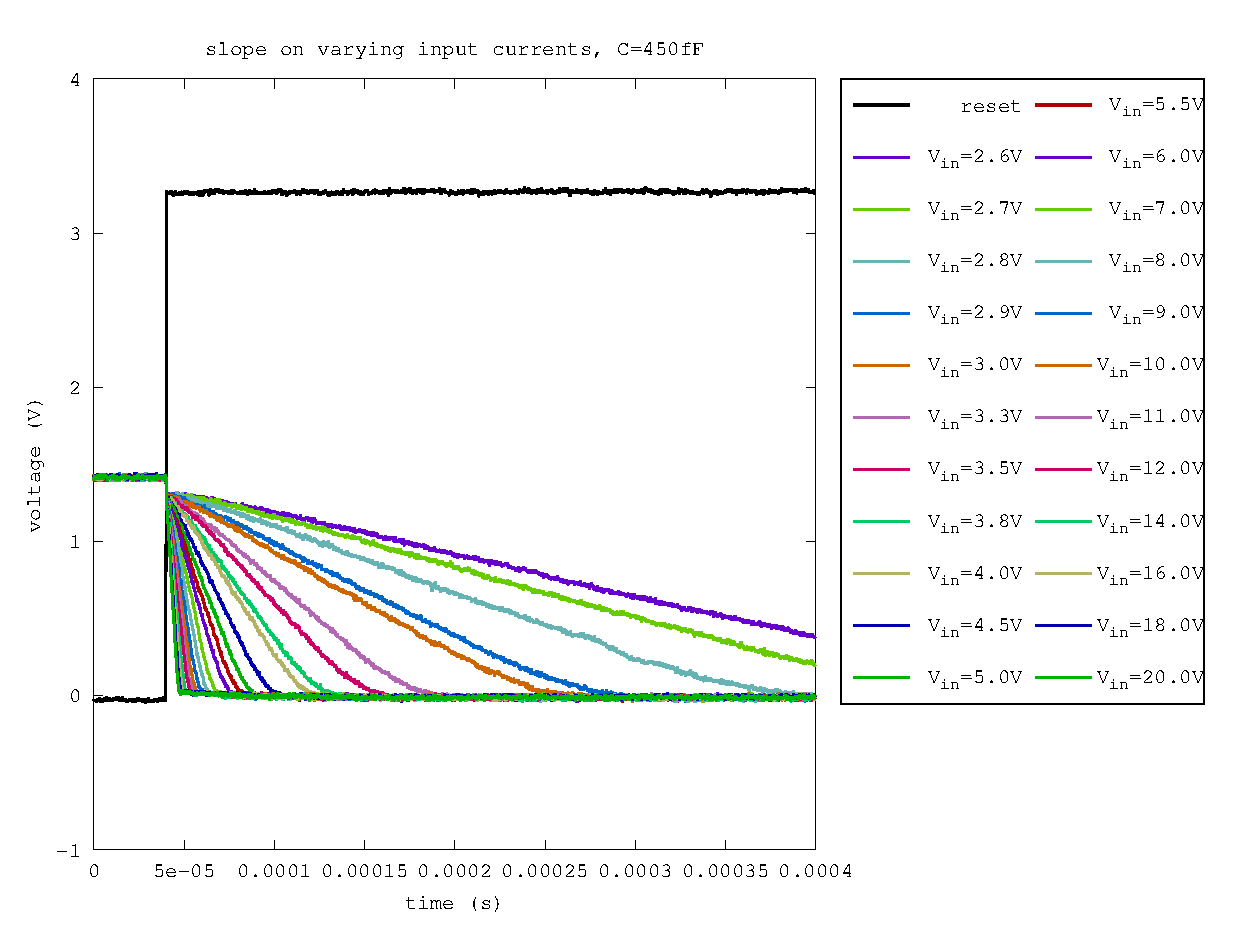
\includegraphics[width=\textwidth]{fig/slope_450fF.eps}
	    \caption[Network2]%
	    {$C=450\,fF$}    
	    \label{fig:slopes_450fF}
	\end{subfigure}
	\hfill
	\begin{subfigure}[b]{0.475\textwidth}  
	    \centering 
	    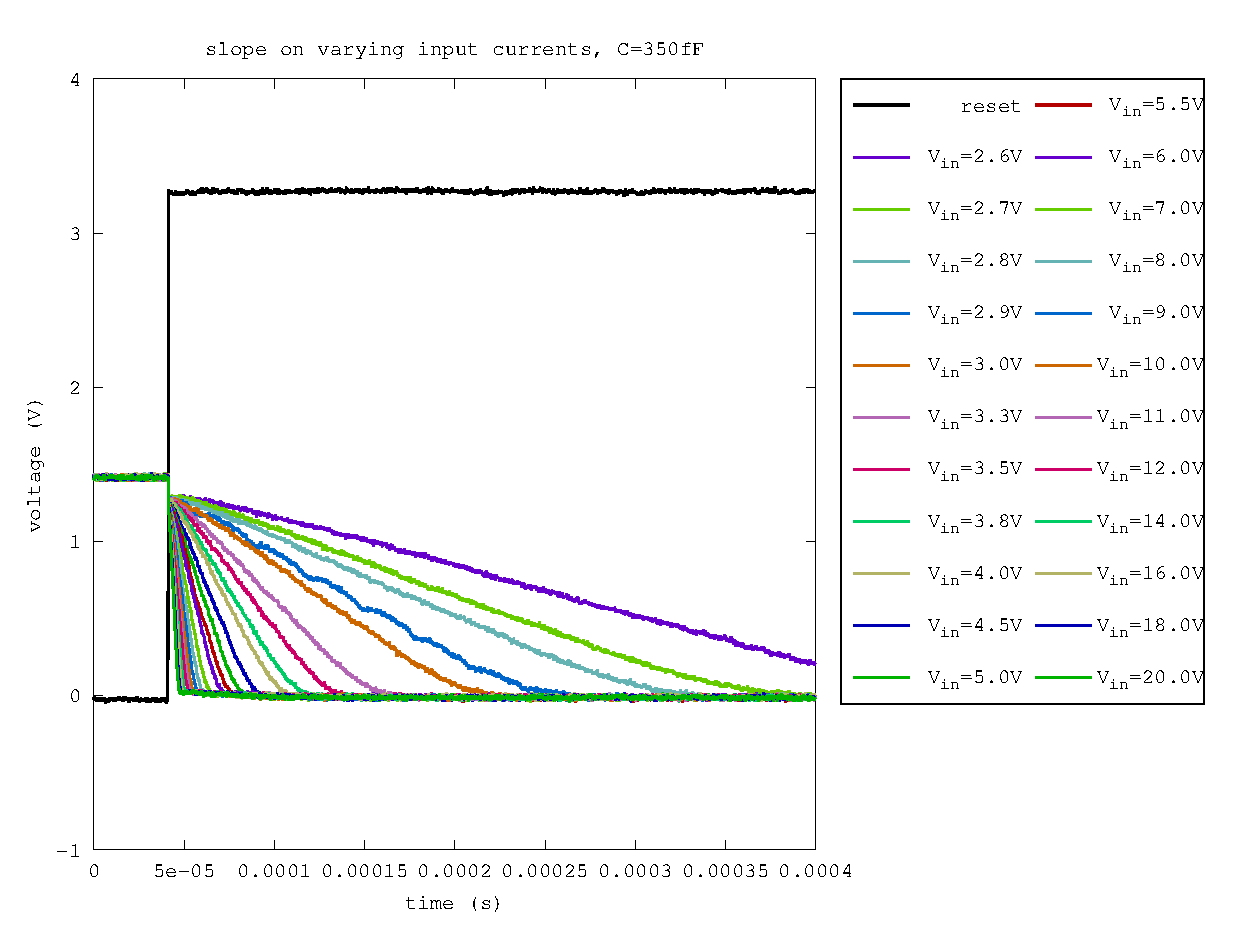
\includegraphics[width=\textwidth]{fig/slope_350fF.eps}
	    \caption[]%
	    {$C=350\,fF$}    
	    \label{fig:slopes_350fF}
	\end{subfigure}
	\vskip\baselineskip
	\begin{subfigure}[b]{0.475\textwidth}   
	    \centering 
	    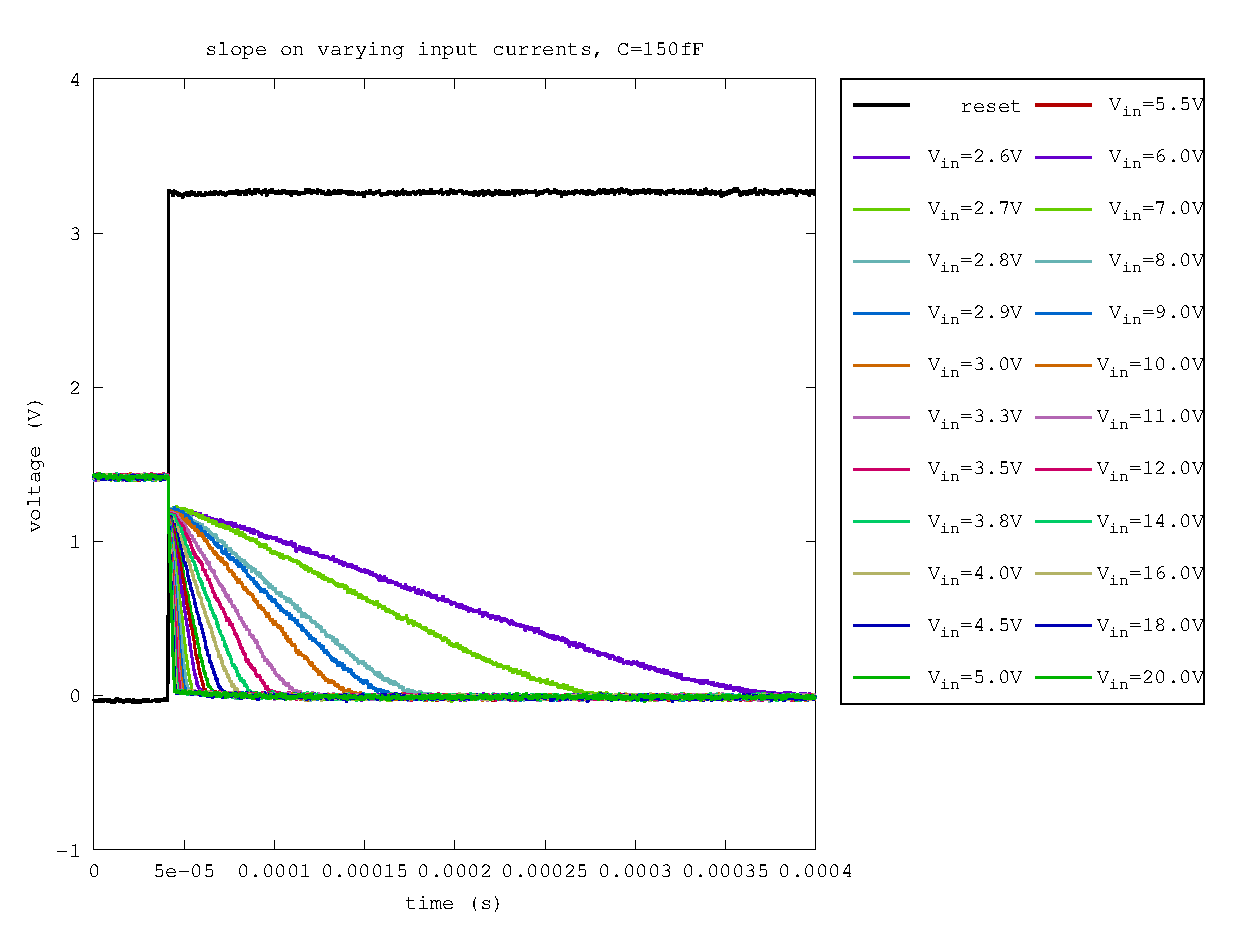
\includegraphics[width=\textwidth]{fig/slope_150fF.eps}
	    \caption[]%
	    {$C=150\,fF$}    
	    \label{fig:slopes_150fF}
	\end{subfigure}
	\quad
	\begin{subfigure}[b]{0.475\textwidth}   
	    \centering 
	    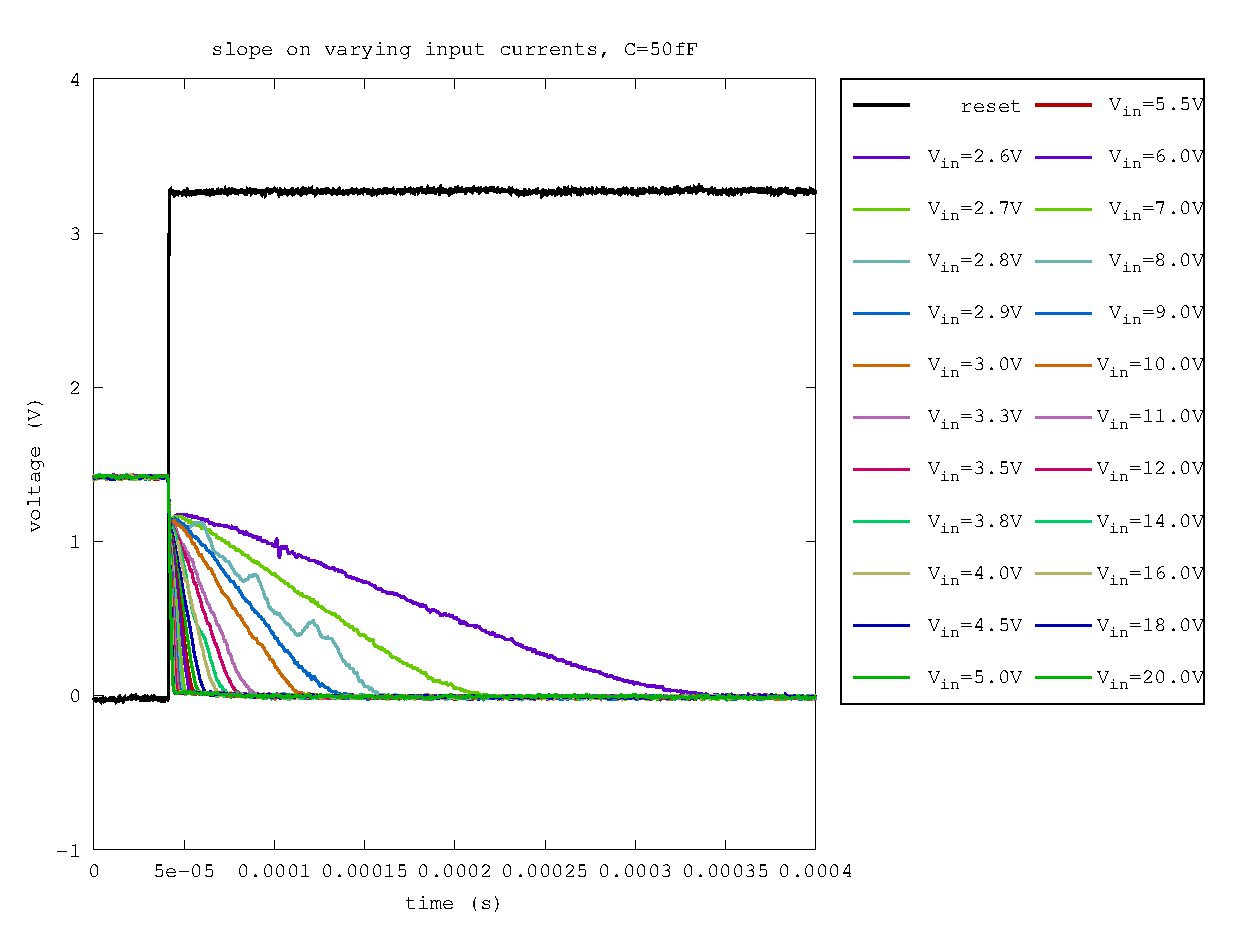
\includegraphics[width=\textwidth]{fig/slope_50fF.eps}
	    \caption[]%
	    {$C=50\,fF$}    
	    \label{fig:slopes_50fF}
	\end{subfigure}
	\caption{Expected versus measured charge up times for different input voltages. The input voltage is connected to the input through a resistor of $20\,M\Omega$}
	\label{fig:slopes}
\end{figure}


\begin{figure}[h]
	\centering
	\begin{subfigure}[b]{0.475\textwidth}
	    \centering
	    \includegraphics[width=\textwidth]{fig/d_slope_450fF.eps}
	    \caption[Network2]%
	    {$C=450\,fF$}    
	    \label{fig:d_slopes_450fF}
	\end{subfigure}
	\hfill
	\begin{subfigure}[b]{0.475\textwidth}  
	    \centering 
	    \includegraphics[width=\textwidth]{fig/d_slope_350fF.eps}
	    \caption[]%
	    {$C=350\,fF$}    
	    \label{fig:d_slopes_350fF}
	\end{subfigure}
	\vskip\baselineskip
	\begin{subfigure}[b]{0.475\textwidth}   
	    \centering 
	    \includegraphics[width=\textwidth]{fig/d_slope_150fF.eps}
	    \caption[]%
	    {$C=150\,fF$}    
	    \label{fig:d_slopes_150fF}
	\end{subfigure}
	\quad
	\begin{subfigure}[b]{0.475\textwidth}   
	    \centering 
	    \includegraphics[width=\textwidth]{fig/d_slope_50fF.eps}
	    \caption[]%
	    {$C=50\,fF$}    
	    \label{fig:d_slopes_50fF}
	\end{subfigure}
	\caption{The plot shows dv/dt against time. The plot is in log scale, which allows for an easy read on the maximum slope and the time needed to discharge the integrator capacitance. }
	\label{fig:d_slopes}
\end{figure}


\begin{figure}[h]
	\centering
	\begin{subfigure}[b]{0.475\textwidth}
	    \centering
	    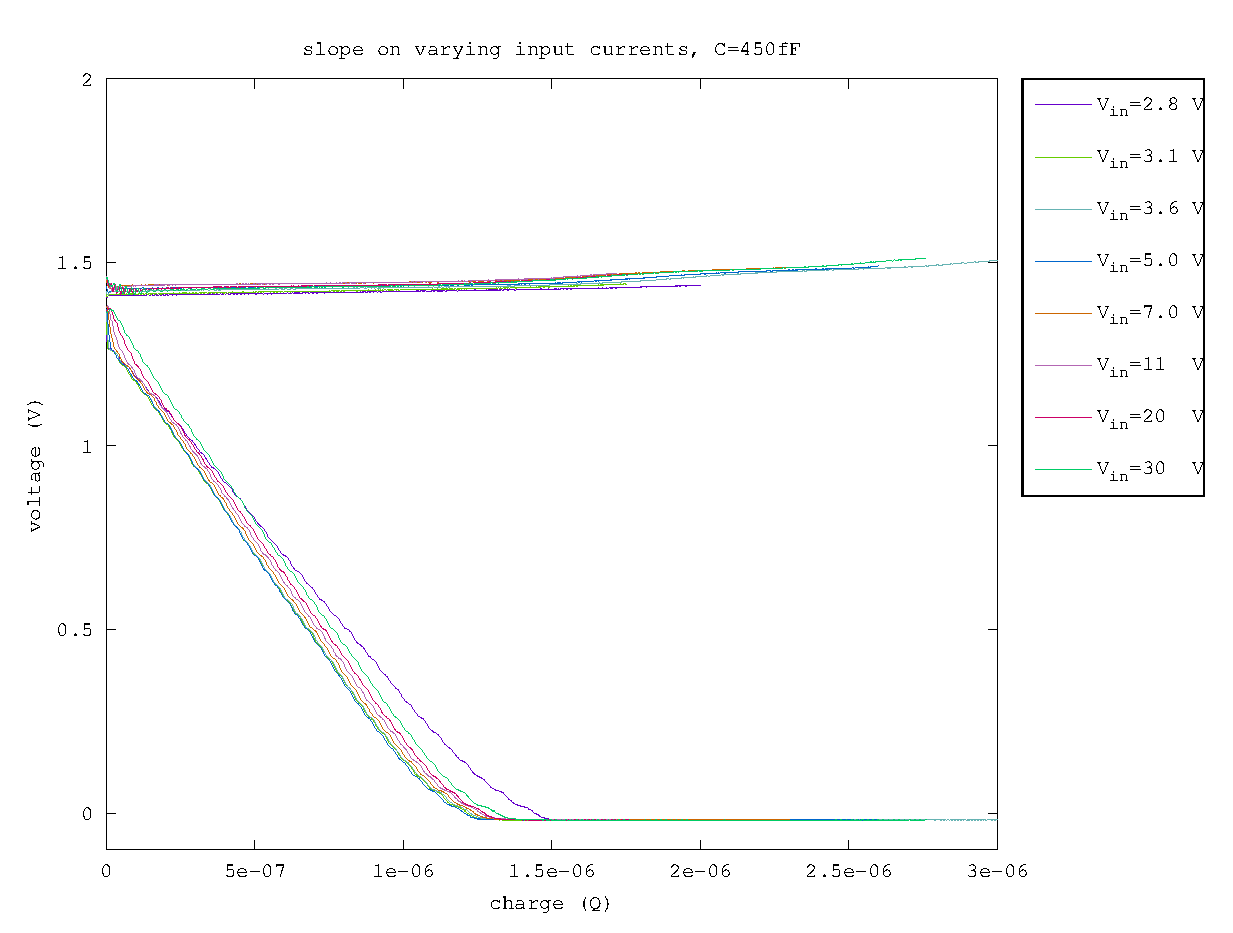
\includegraphics[width=\textwidth]{fig/charge_450fF.eps}
	    \caption[Network2]%
	    {$C=450\,fF$}    
	    \label{fig:charges_450fF}
	\end{subfigure}
	\hfill
	\begin{subfigure}[b]{0.475\textwidth}  
	    \centering 
	    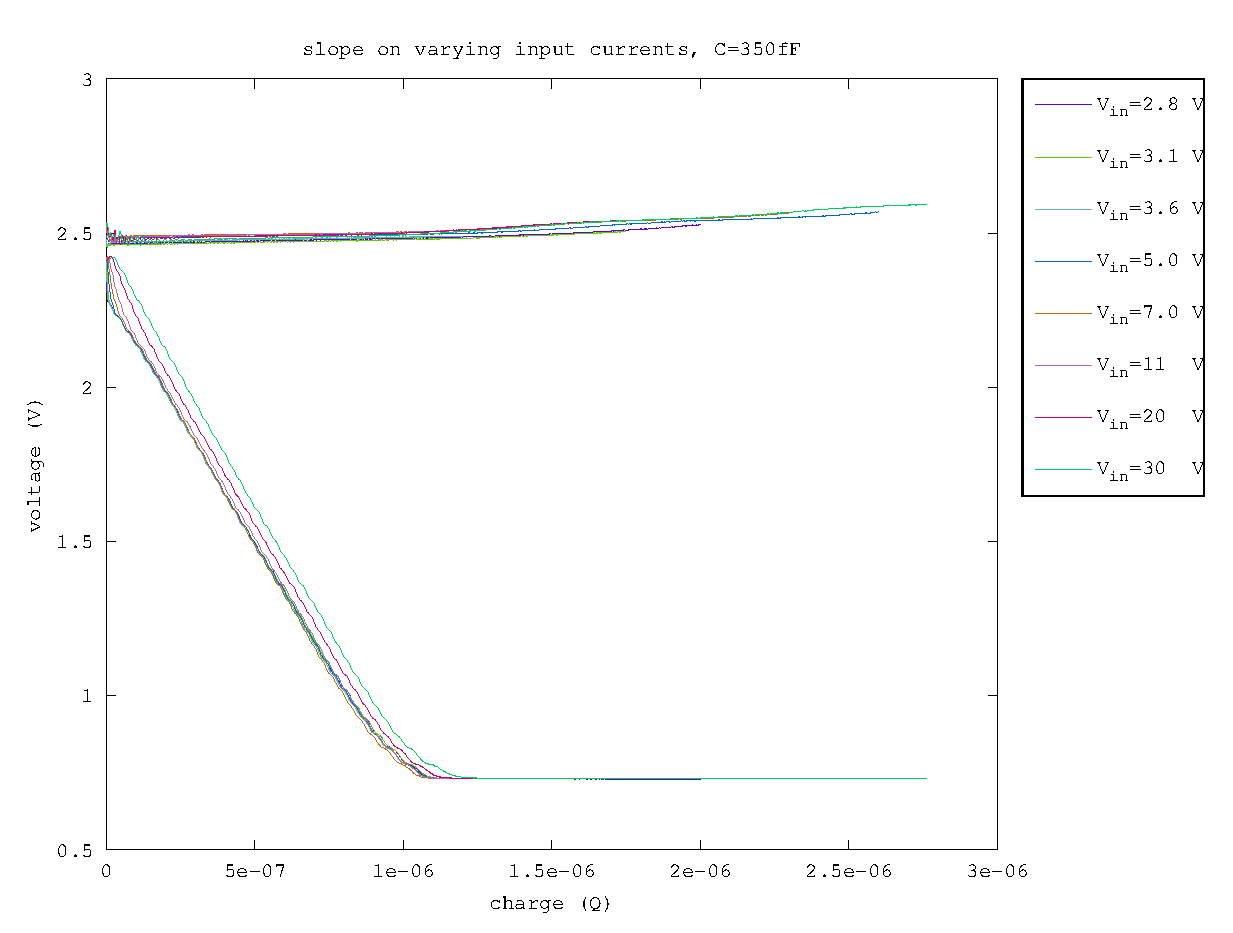
\includegraphics[width=\textwidth]{fig/charge_350fF.eps}
	    \caption[]%
	    {$C=350\,fF$}    
	    \label{fig:charges_350fF}
	\end{subfigure}
	\vskip\baselineskip
	\begin{subfigure}[b]{0.475\textwidth}   
	    \centering 
	    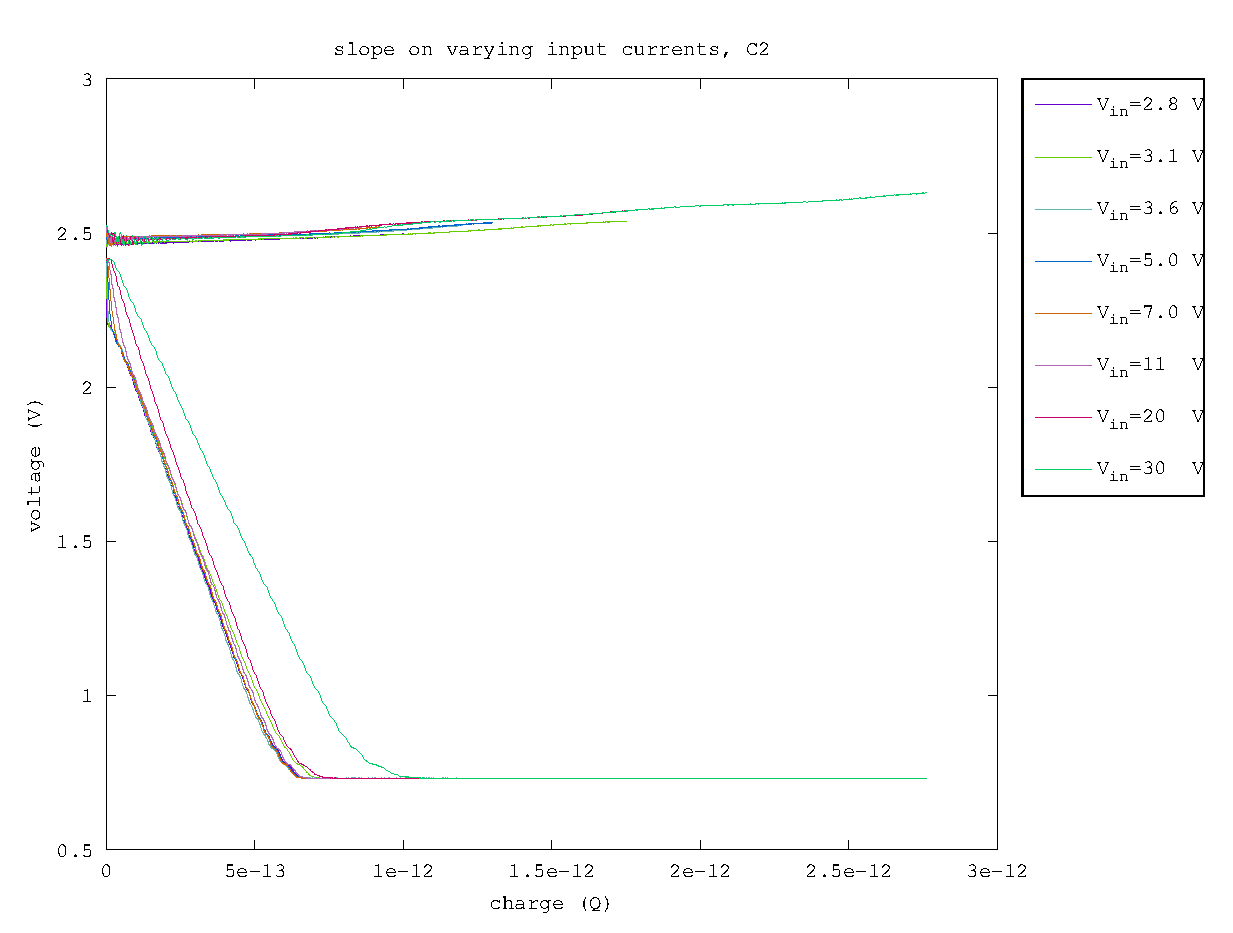
\includegraphics[width=\textwidth]{fig/charge_150fF.eps}
	    \caption[]%
	    {$C=150\,fF$}    
	    \label{fig:charges_150fF}
	\end{subfigure}
	\quad
	\begin{subfigure}[b]{0.475\textwidth}   
	    \centering 
	    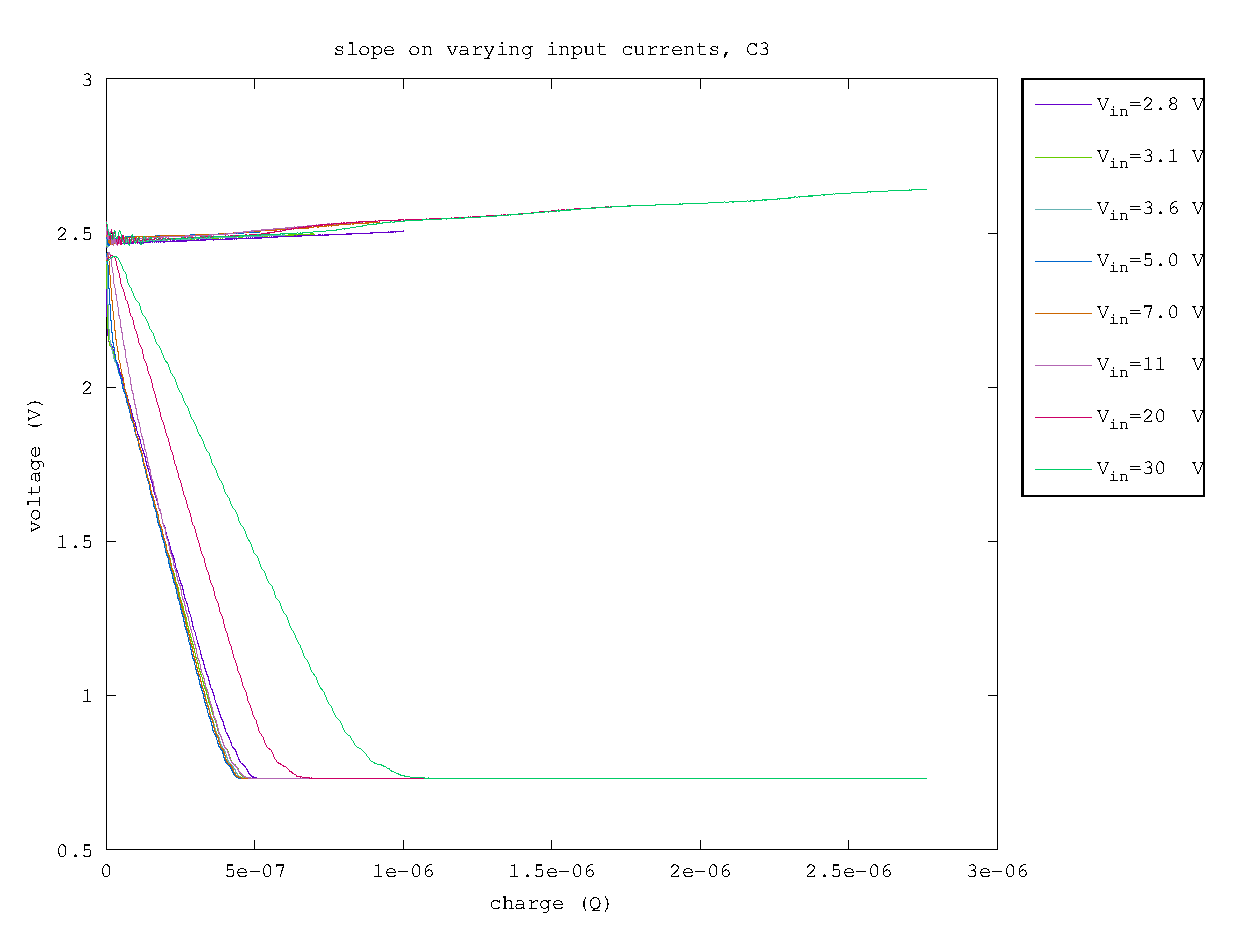
\includegraphics[width=\textwidth]{fig/charge_50fF.eps}
	    \caption[]%
	    {$C=50\,fF$}    
	    \label{fig:charges_50fF}
	\end{subfigure}
	\caption{This plot is showing charge versus voltage}
	\label{fig:charges}
\end{figure}

\begin{figure}[h]
	\centering
	\begin{subfigure}[b]{0.475\textwidth}
	    \centering
	    \includegraphics[width=\textwidth]{fig/vin_vs_time_sat_450fF.eps}
	    \caption[Network2]%
	    {$C=450\,fF$}    
	    \label{fig:e_vs_m_450fF}
	\end{subfigure}
	\hfill
	\begin{subfigure}[b]{0.475\textwidth}  
	    \centering 
	    \includegraphics[width=\textwidth]{fig/vin_vs_time_sat_350fF.eps}
	    \caption[]%
	    {$C=350\,fF$}    
	    \label{fig:e_vs_m_350fF}
	\end{subfigure}
	\vskip\baselineskip
	\begin{subfigure}[b]{0.475\textwidth}   
	    \centering 
	    \includegraphics[width=\textwidth]{fig/vin_vs_time_sat_150fF.eps}
	    \caption[]%
	    {$C=150\,fF$}    
	    \label{fig:e_vs_m_150fF}
	\end{subfigure}
	\quad
	\begin{subfigure}[b]{0.475\textwidth}   
	    \centering 
	    \includegraphics[width=\textwidth]{fig/vin_vs_time_sat_50fF.eps}
	    \caption[]%
	    {$C=50\,fF$}    
	    \label{fig:e_vs_m_50fF}
	\end{subfigure}
	\caption{Expected versus measured charge up times for different input voltages. The input voltage is connected to the input through a resistor of $20\,M\Omega$.}
	\label{fig:e_vs_m}
\end{figure}

\clearpage
\section{large current  focussed}
In this section the $20\,M\Omega$ input resistor is replaecd with a $4\,M\Omega$ resistor.
\begin{figure}[h]
	\centering
	\begin{subfigure}[b]{0.475\textwidth}
	    \centering
	    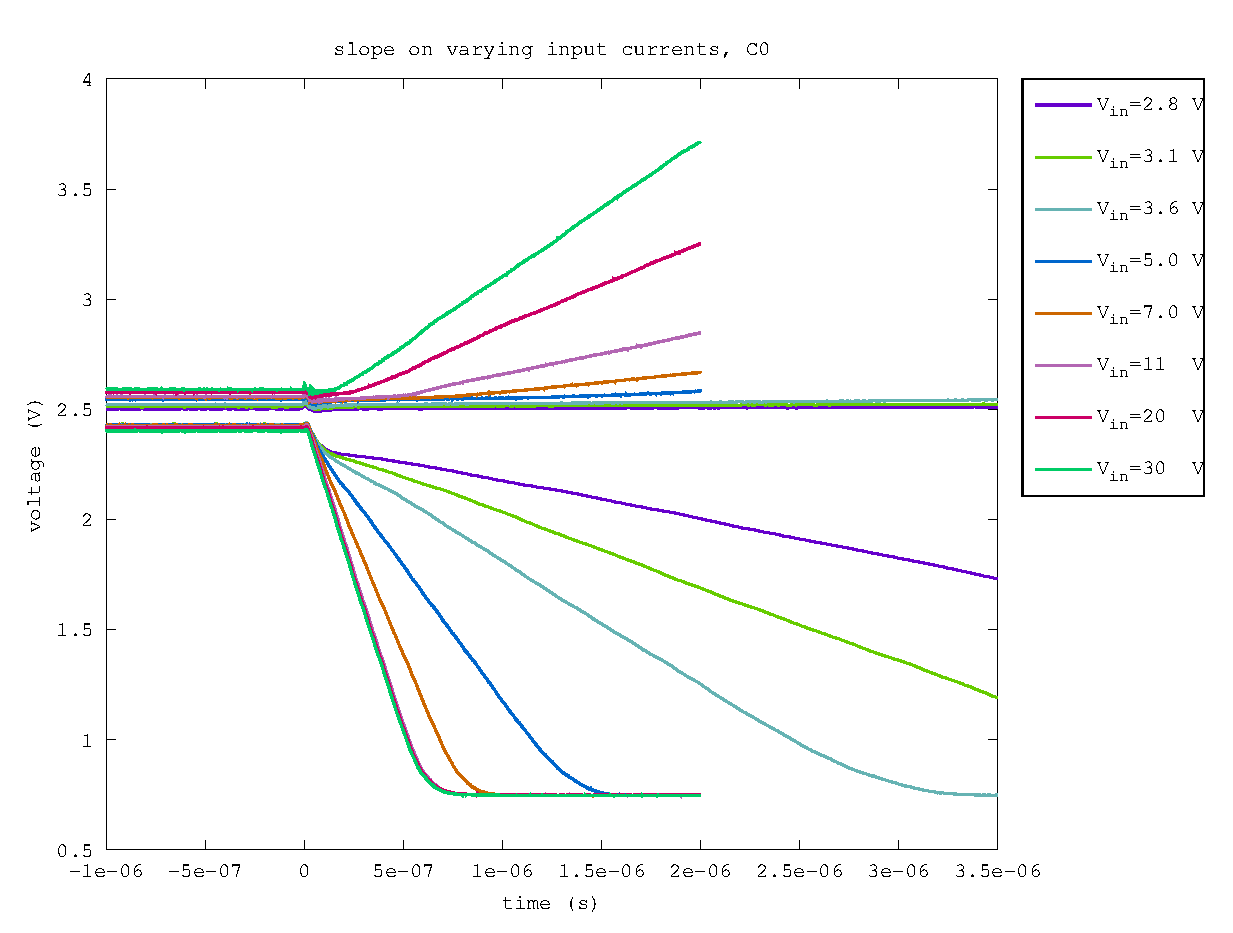
\includegraphics[width=\textwidth]{fig/bre_slope_450fF.eps}
	    \caption[Network2]%
	    {$C=450\,fF$}    
	    \label{fig:bre_slopes_450fF}
	\end{subfigure}
	\hfill
	\begin{subfigure}[b]{0.475\textwidth}  
	    \centering 
	    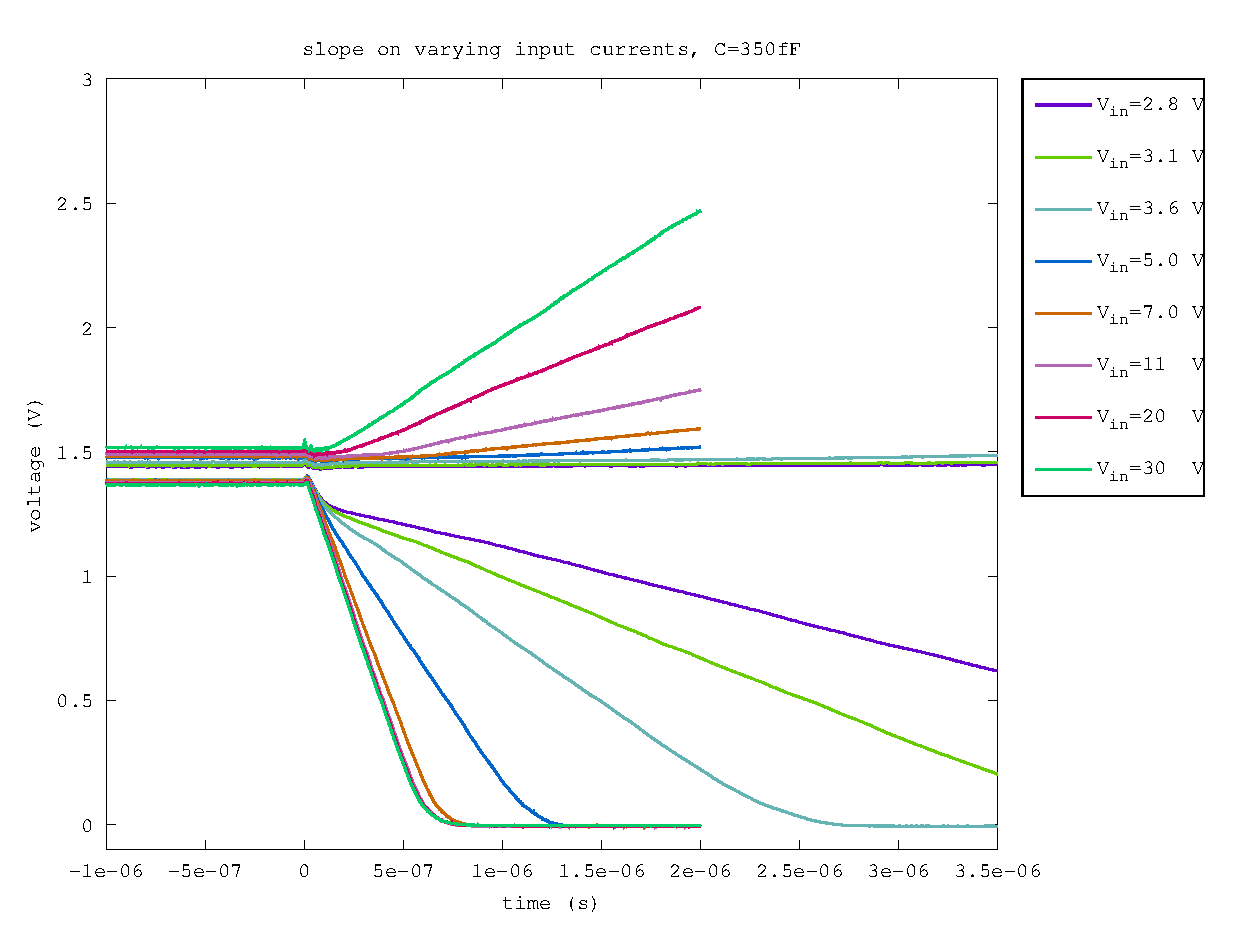
\includegraphics[width=\textwidth]{fig/bre_slope_350fF.eps}
	    \caption[]%
	    {$C=350\,fF$}    
	    \label{fig:bre_slopes_350fF}
	\end{subfigure}
	\vskip\baselineskip
	\begin{subfigure}[b]{0.475\textwidth}   
	    \centering 
	    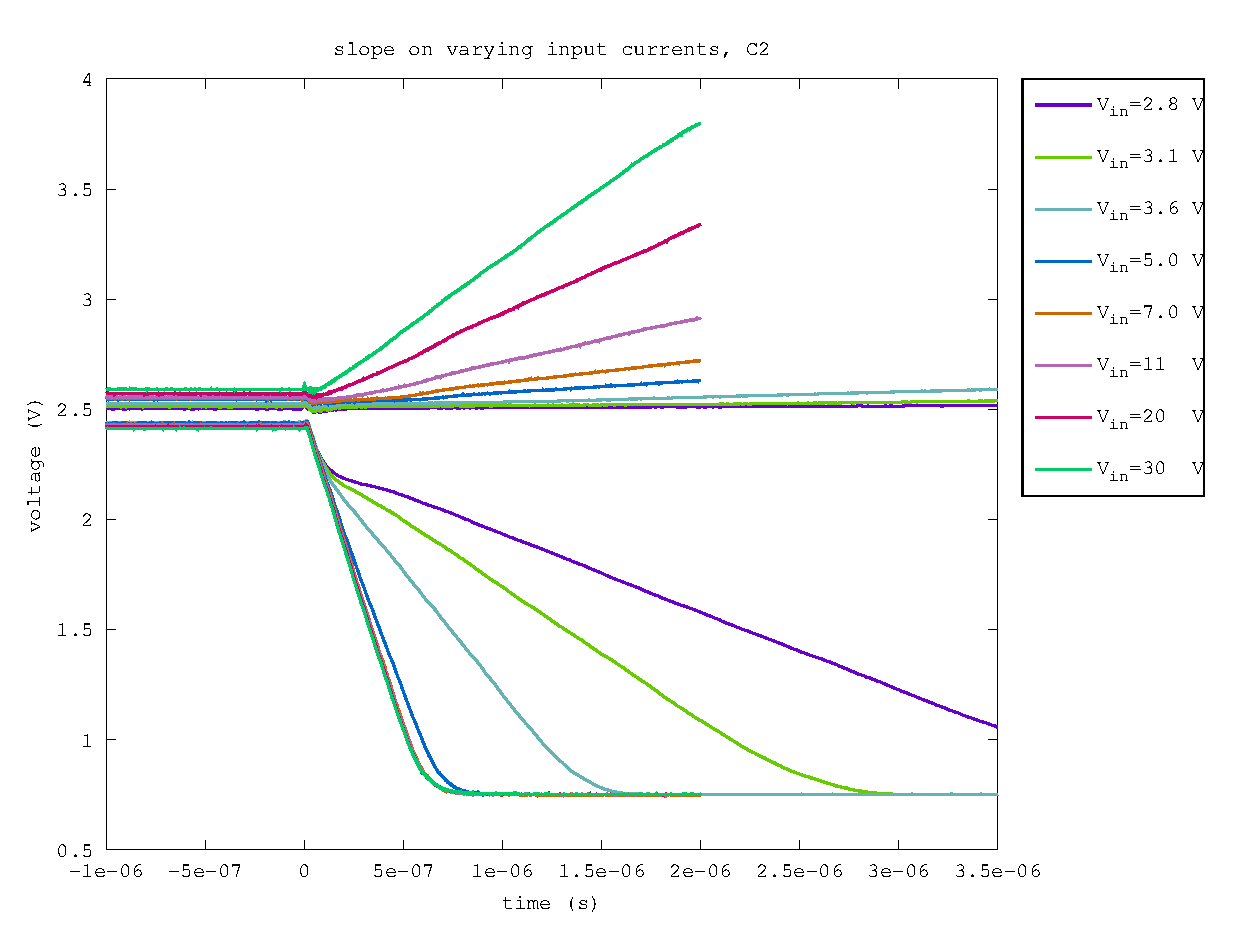
\includegraphics[width=\textwidth]{fig/bre_slope_150fF.eps}
	    \caption[]%
	    {$C=150\,fF$}    
	    \label{fig:bre_slopes_150fF}
	\end{subfigure}
	\quad
	\begin{subfigure}[b]{0.475\textwidth}   
	    \centering 
	    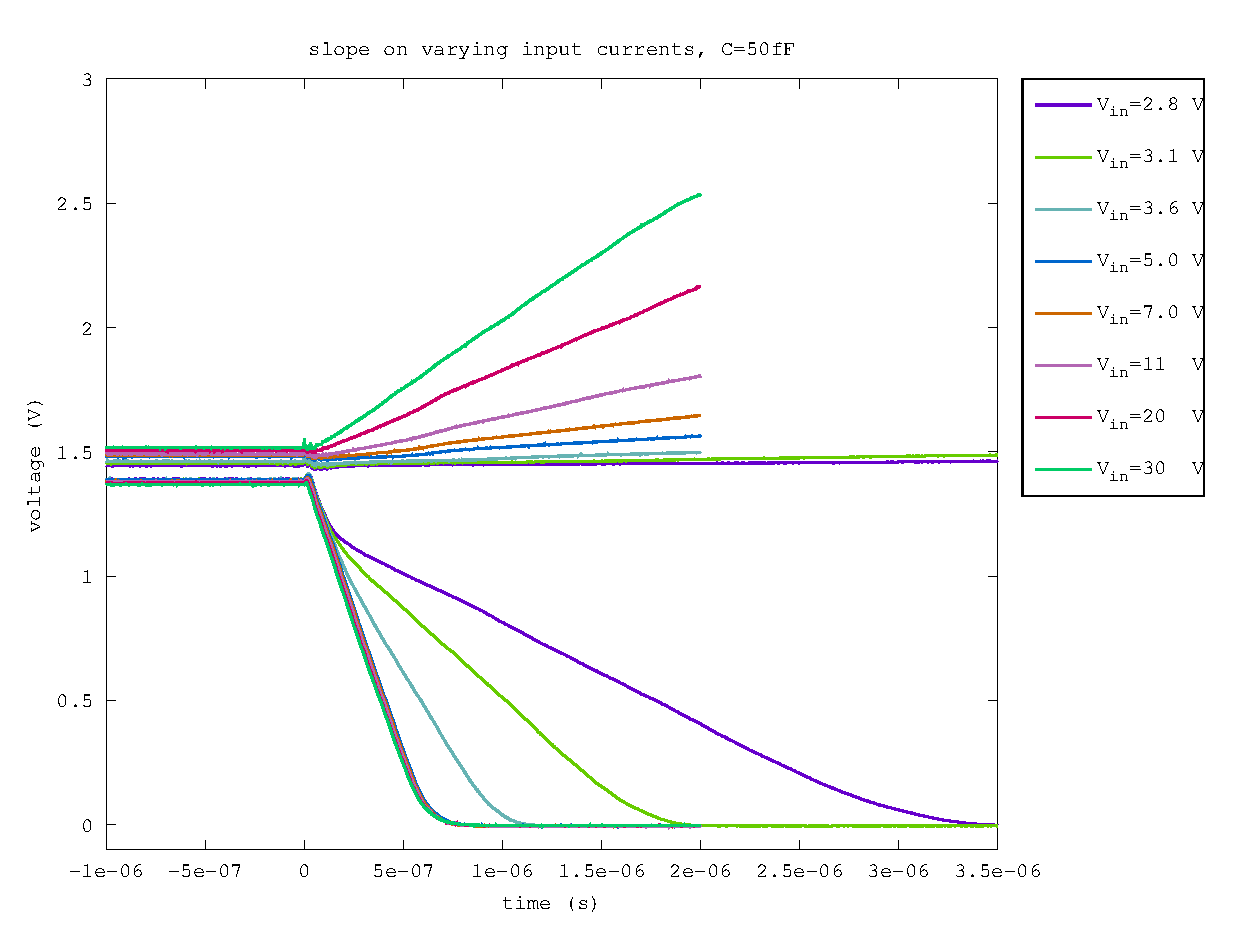
\includegraphics[width=\textwidth]{fig/bre_slope_50fF.eps}
	    \caption[]%
	    {$C=50\,fF$}    
	    \label{fig:bre_slopes_50fF}
	\end{subfigure}
	\caption{Expected versus measured charge up times for different input voltages. The input voltage is connected to the input through a resistor of $4\,M\Omega$}
	\label{fig:bre_slopes}
\end{figure}


\begin{figure}[h]
	\centering
	\begin{subfigure}[b]{0.475\textwidth}
	    \centering
	    \includegraphics[width=\textwidth]{fig/bre_d_slope_450fF.eps}
	    \caption[Network2]%
	    {$C=450\,fF$}    
	    \label{fig:bre_d_slopes_450fF}
	\end{subfigure}
	\hfill
	\begin{subfigure}[b]{0.475\textwidth}  
	    \centering 
	    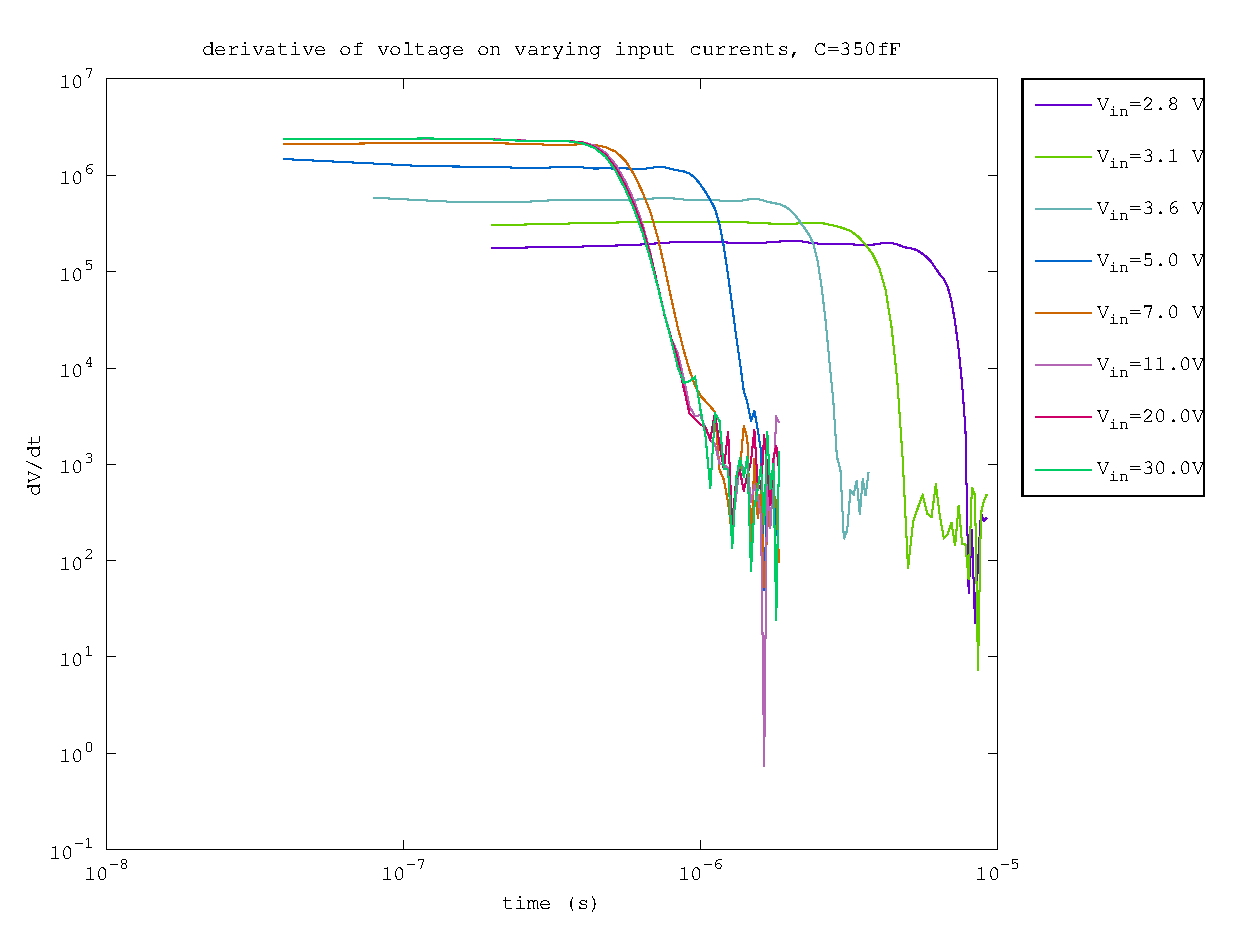
\includegraphics[width=\textwidth]{fig/bre_d_slope_350fF.eps}
	    \caption[]%
	    {$C=350\,fF$}    
	    \label{fig:bre_d_slopes_350fF}
	\end{subfigure}
	\vskip\baselineskip
	\begin{subfigure}[b]{0.475\textwidth}   
	    \centering 
	    \includegraphics[width=\textwidth]{fig/bre_d_slope_150fF.eps}
	    \caption[]%
	    {$C=150\,fF$}    
	    \label{fig:bre_d_slopes_150fF}
	\end{subfigure}
	\quad
	\begin{subfigure}[b]{0.475\textwidth}   
	    \centering 
	    \includegraphics[width=\textwidth]{fig/bre_d_slope_50fF.eps}
	    \caption[]%
	    {$C=50\,fF$}    
	    \label{fig:bre_d_slopes_50fF}
	\end{subfigure}
	\caption{The plot shows dv/dt against time. The plot is in log scale, which allows for an easy read on the maximum slope and the time needed to discharge the integrator capacitance. }
	\label{fig:bre_d_slopes}
\end{figure}


\begin{figure}[h]
	\centering
	\begin{subfigure}[b]{0.475\textwidth}
	    \centering
	    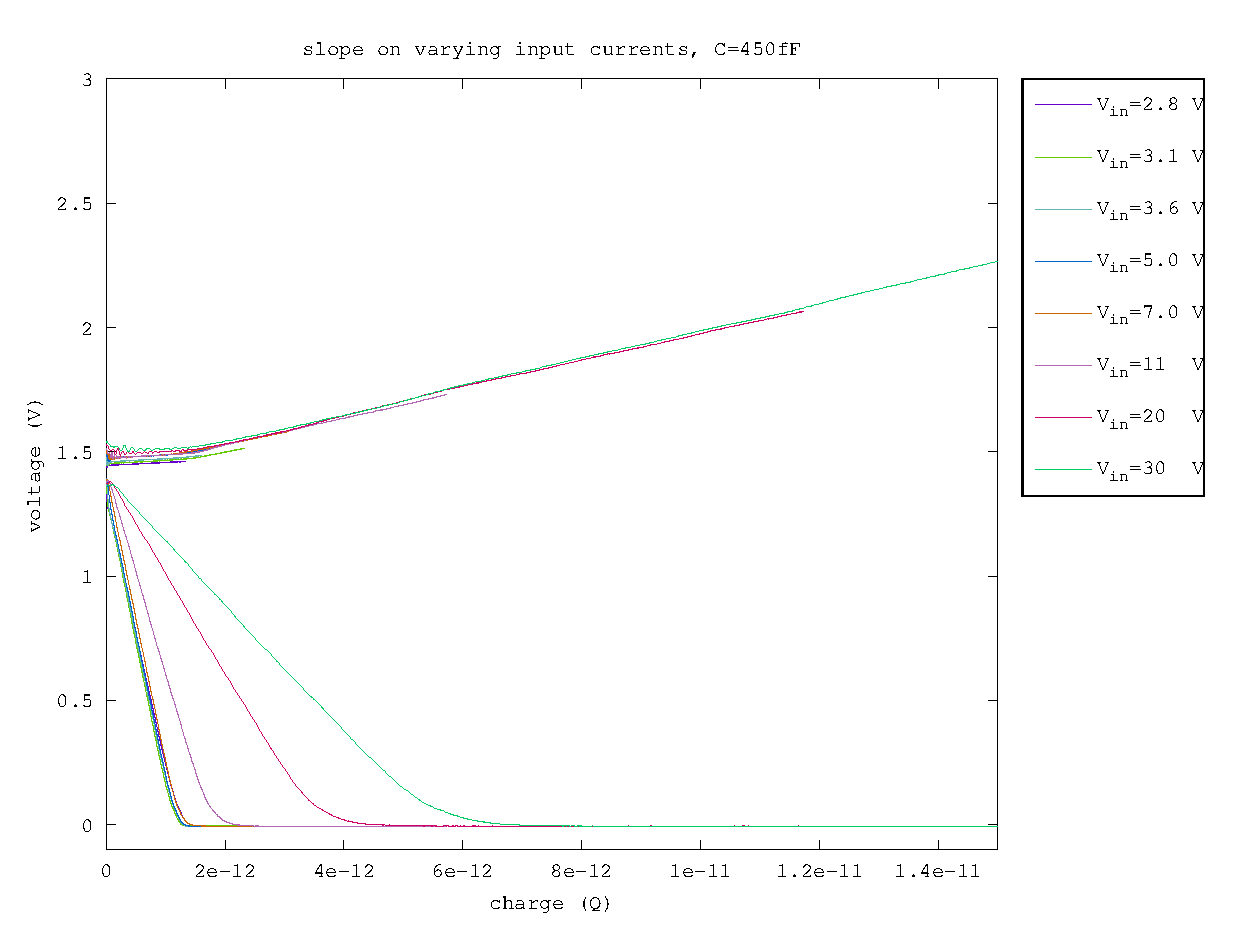
\includegraphics[width=\textwidth]{fig/bre_charge_450fF.eps}
	    \caption[Network2]%
	    {$C=450\,fF$}    
	    \label{fig:bre_charges_450fF}
	\end{subfigure}
	\hfill
	\begin{subfigure}[b]{0.475\textwidth}  
	    \centering 
	    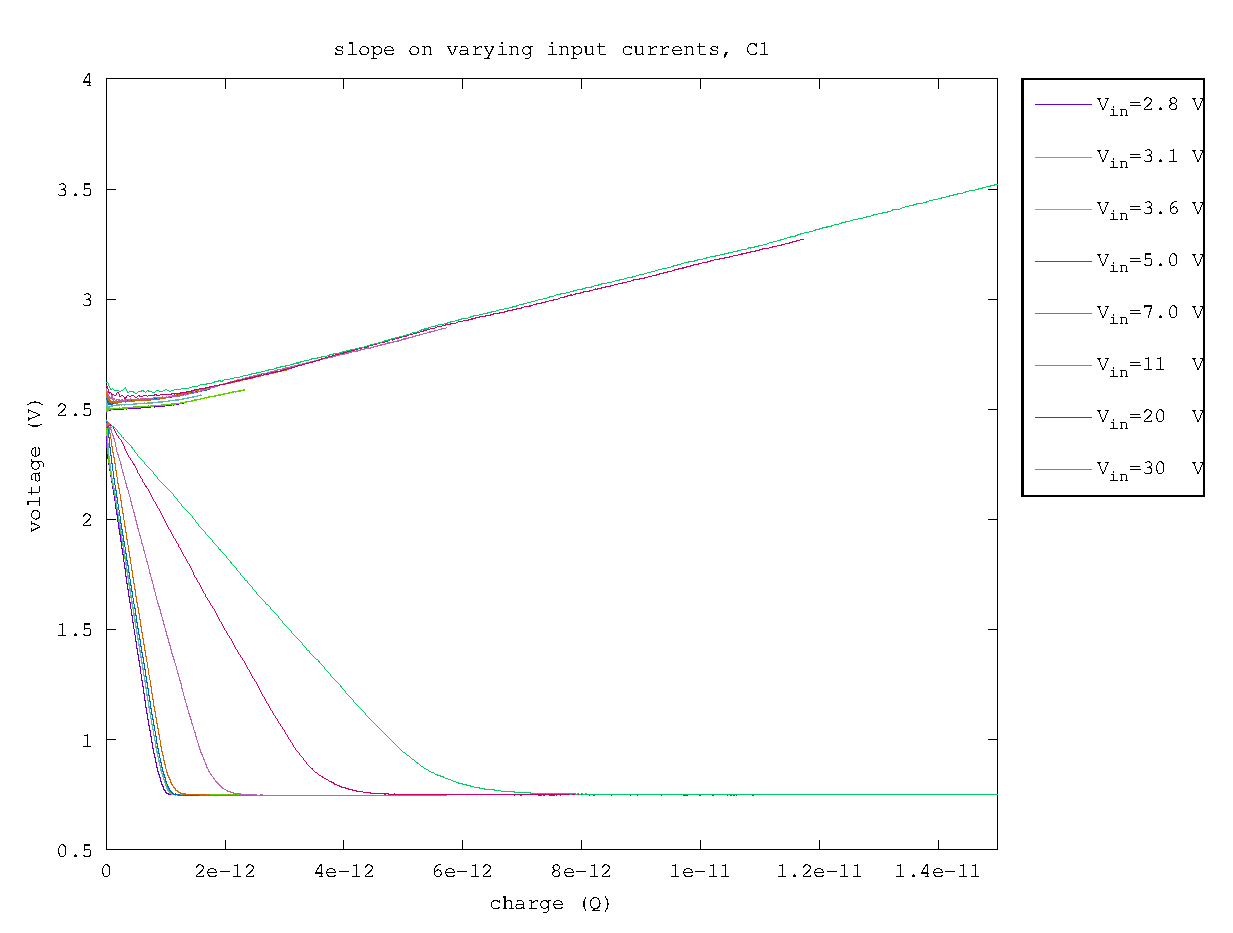
\includegraphics[width=\textwidth]{fig/bre_charge_350fF.eps}
	    \caption[]%
	    {$C=350\,fF$}    
	    \label{fig:bre_charges_350fF}
	\end{subfigure}
	\vskip\baselineskip
	\begin{subfigure}[b]{0.475\textwidth}   
	    \centering 
	    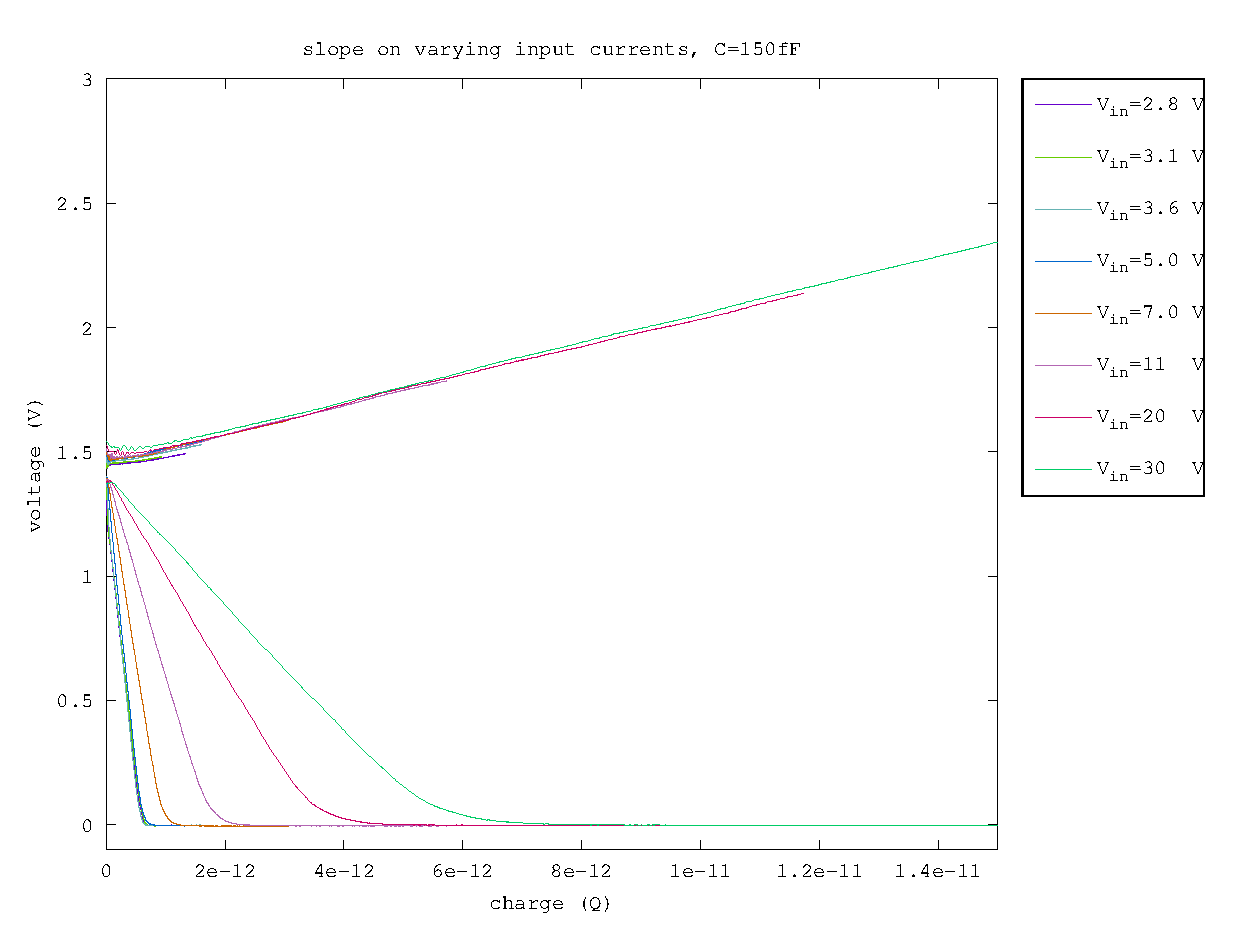
\includegraphics[width=\textwidth]{fig/bre_charge_150fF.eps}
	    \caption[]%
	    {$C=150\,fF$}    
	    \label{fig:bre_charges_150fF}
	\end{subfigure}
	\quad
	\begin{subfigure}[b]{0.475\textwidth}   
	    \centering 
	    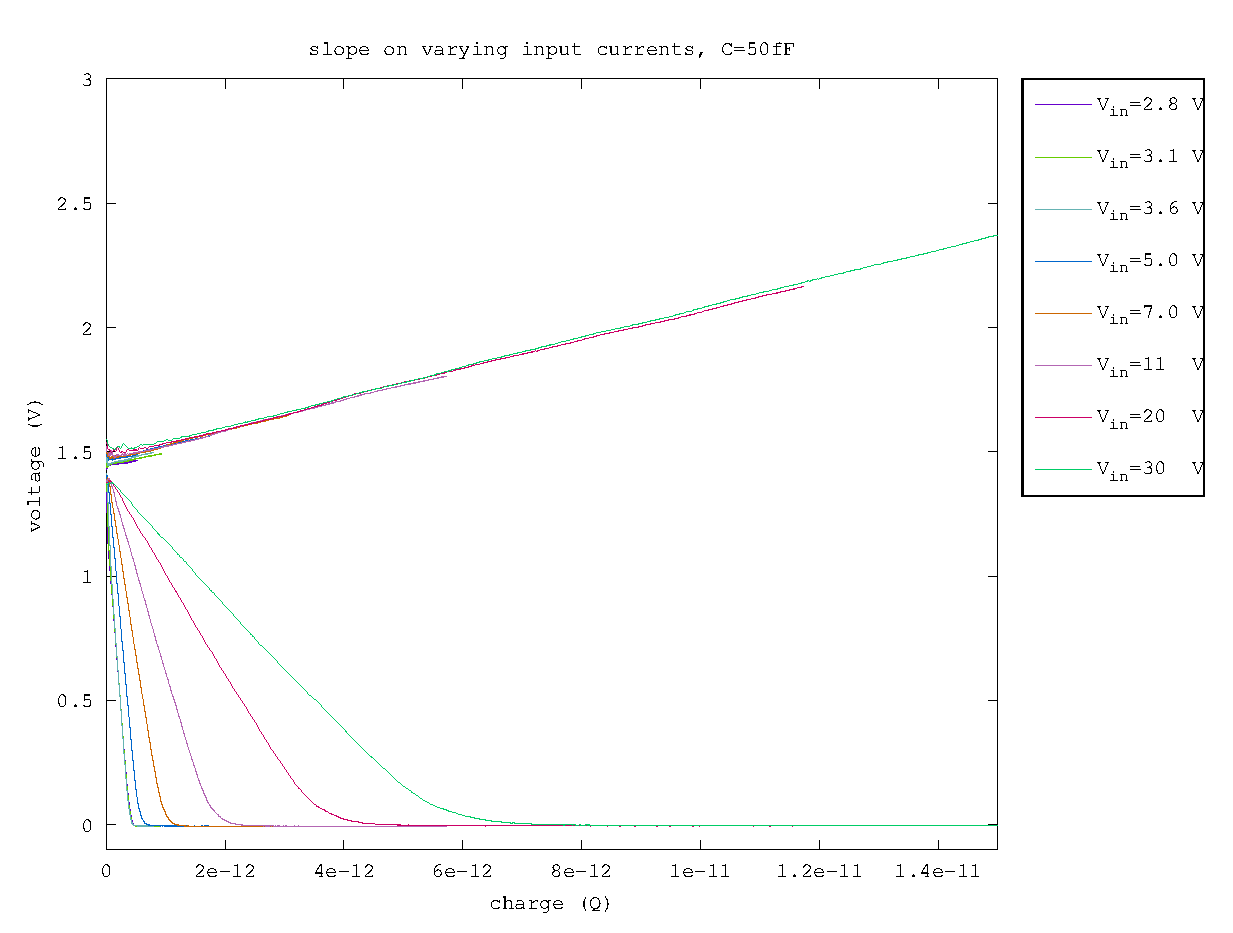
\includegraphics[width=\textwidth]{fig/bre_charge_50fF.eps}
	    \caption[]%
	    {$C=50\,fF$}    
	    \label{fig:bre_charges_50fF}
	\end{subfigure}
	\caption{This plot is showing charge versus voltage}
	\label{fig:bre_charges}
\end{figure}

\begin{figure}[h]
	\centering
	\begin{subfigure}[b]{0.475\textwidth}
	    \centering
	    \includegraphics[width=\textwidth]{fig/bre_vin_vs_time_sat_450fF.eps}
	    \caption[Network2]%
	    {$C=450\,fF$}    
	    \label{fig:bre_e_vs_m_450fF}
	\end{subfigure}
	\hfill
	\begin{subfigure}[b]{0.475\textwidth}  
	    \centering 
	    \includegraphics[width=\textwidth]{fig/bre_vin_vs_time_sat_350fF.eps}
	    \caption[]%
	    {$C=350\,fF$}    
	    \label{fig:bre_e_vs_m_350fF}
	\end{subfigure}
	\vskip\baselineskip
	\begin{subfigure}[b]{0.475\textwidth}   
	    \centering 
	    \includegraphics[width=\textwidth]{fig/bre_vin_vs_time_sat_150fF.eps}
	    \caption[]%
	    {$C=150\,fF$}    
	    \label{fig:bre_e_vs_m_150fF}
	\end{subfigure}
	\quad
	\begin{subfigure}[b]{0.475\textwidth}   
	    \centering 
	    \includegraphics[width=\textwidth]{fig/bre_vin_vs_time_sat_50fF.eps}
	    \caption[]%
	    {$C=50\,fF$}    
	    \label{fig:bre_e_vs_m_50fF}
	\end{subfigure}
	\caption{Expected versus measured charge up times for different input voltages. The input voltage is connected to the input through a resistor of $4\,M\Omega$.}
	\label{fig:bre_e_vs_m}
\end{figure}



\clearpage
\section{vbo  focussed}

\begin{figure}[h]
	\centering
	\begin{subfigure}[b]{0.475\textwidth}
	    \centering
	    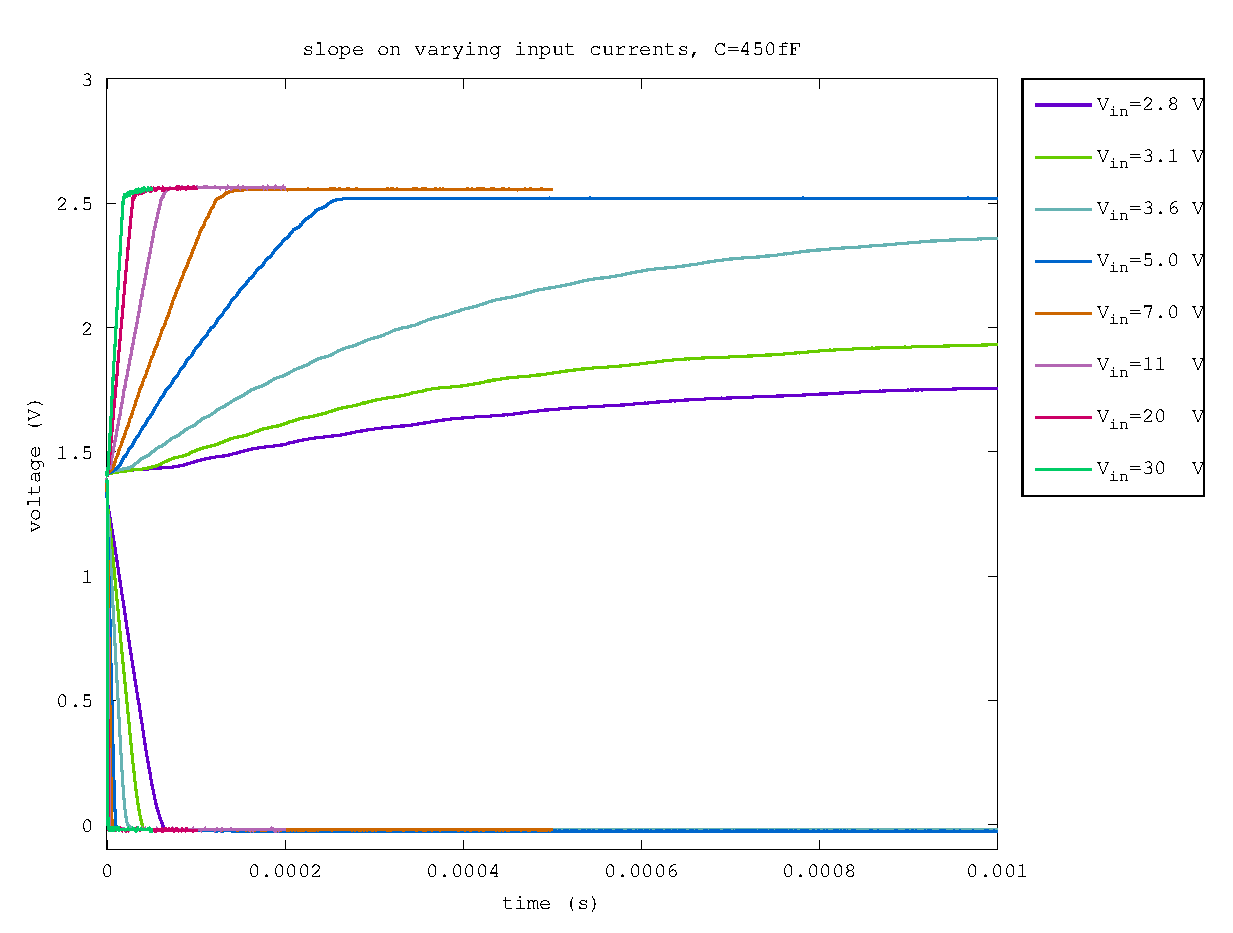
\includegraphics[width=\textwidth]{fig/vbo_slope_450fF.eps}
	    \caption[Network2]%
	    {$C=450\,fF$}    
	    \label{fig:vbo_slopes_450fF}
	\end{subfigure}
	\hfill
	\begin{subfigure}[b]{0.475\textwidth}  
	    \centering 
	    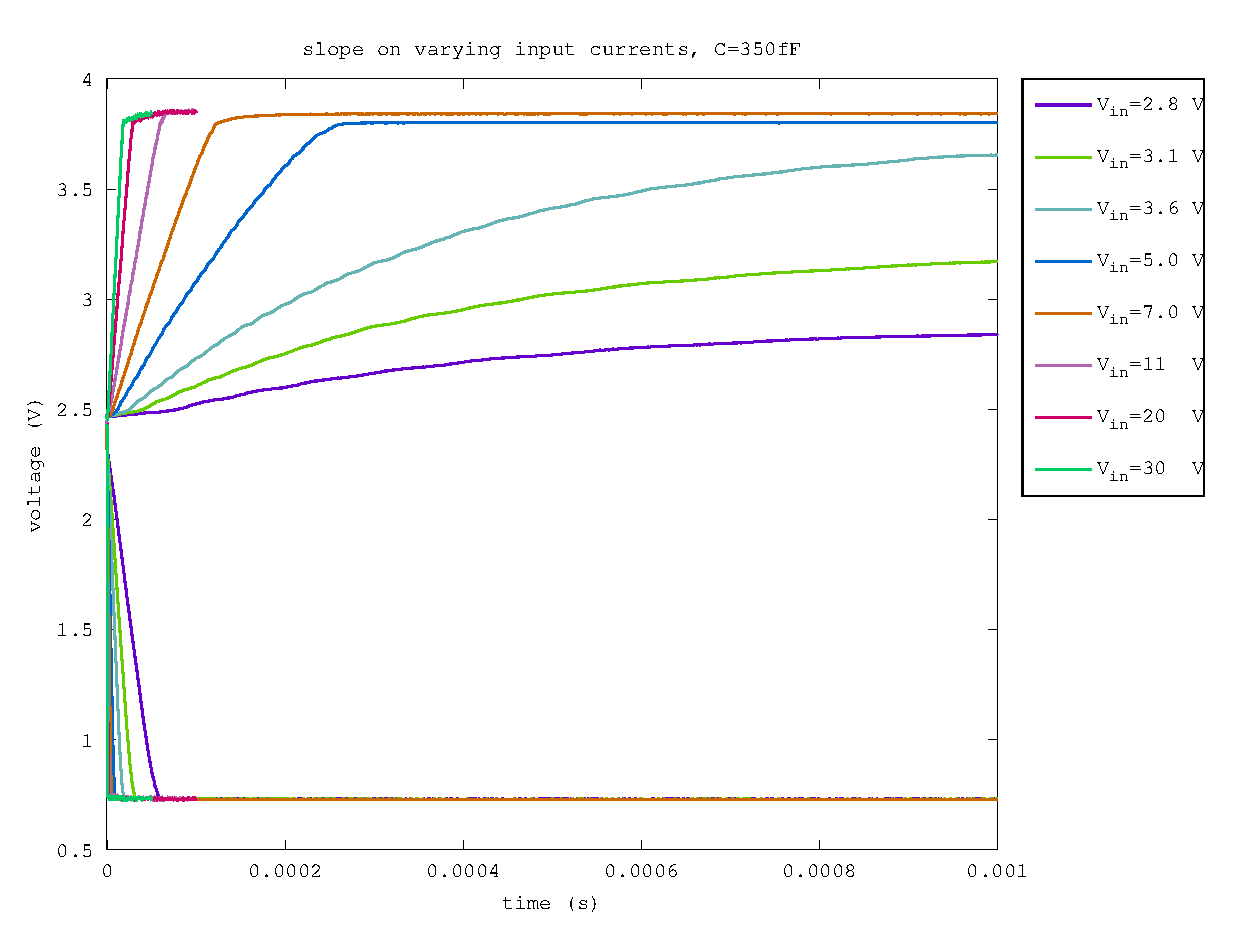
\includegraphics[width=\textwidth]{fig/vbo_slope_350fF.eps}
	    \caption[]%
	    {$C=350\,fF$}    
	    \label{fig:vbo_slopes_350fF}
	\end{subfigure}
	\vskip\baselineskip
	\begin{subfigure}[b]{0.475\textwidth}   
	    \centering 
	    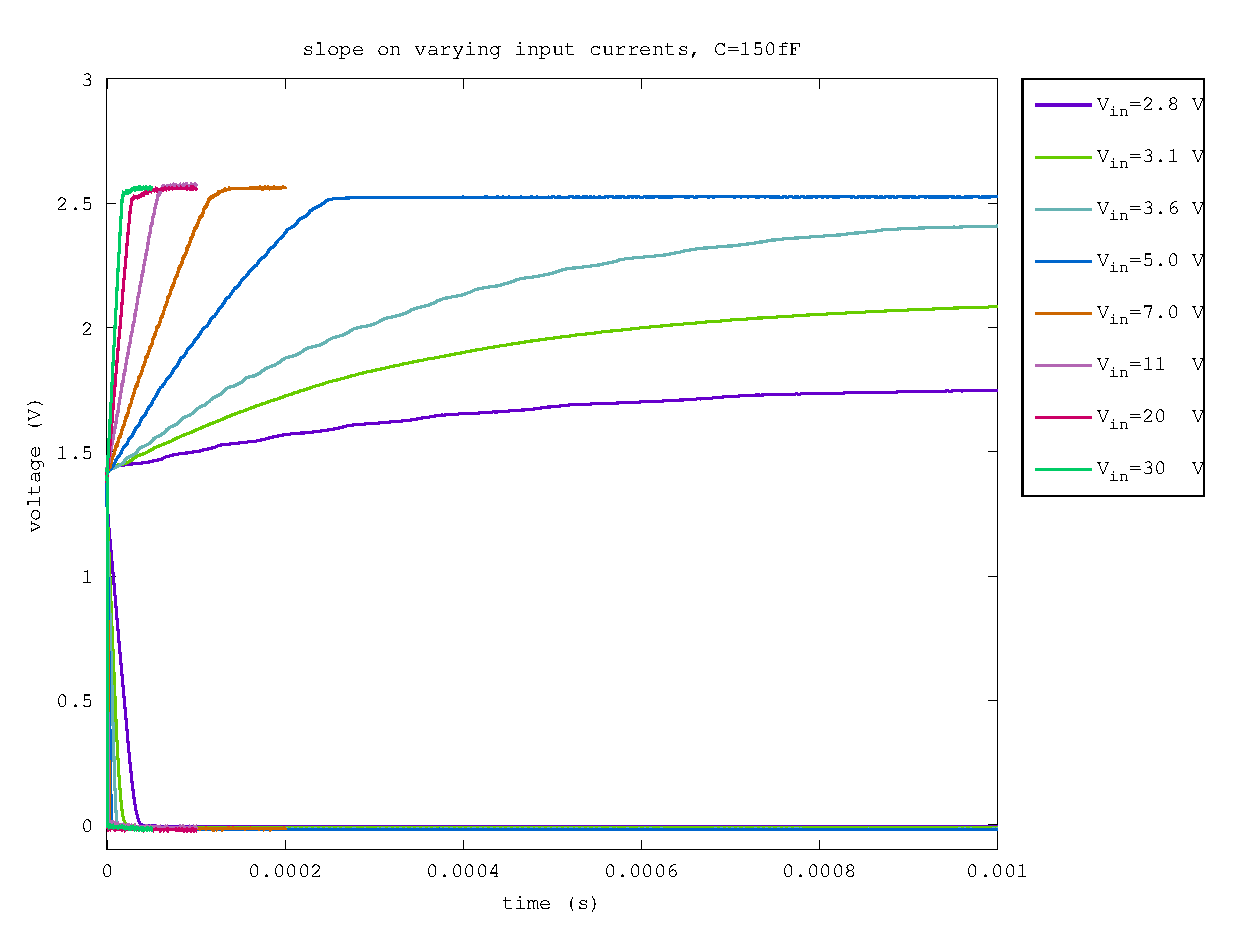
\includegraphics[width=\textwidth]{fig/vbo_slope_150fF.eps}
	    \caption[]%
	    {$C=150\,fF$}    
	    \label{fig:vbo_slopes_150fF}
	\end{subfigure}
	\quad
	\begin{subfigure}[b]{0.475\textwidth}   
	    \centering 
	    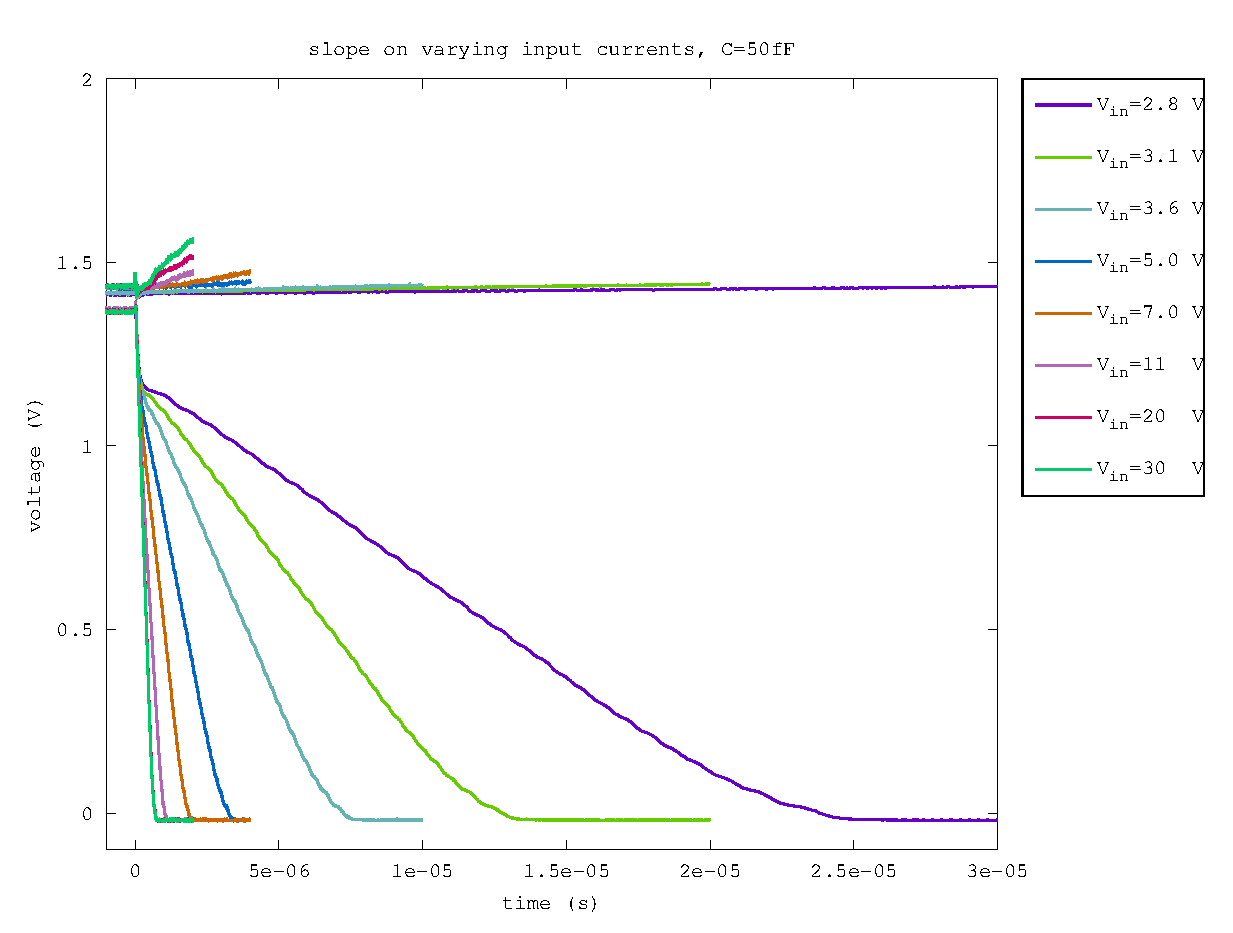
\includegraphics[width=\textwidth]{fig/vbo_slope_50fF.eps}
	    \caption[]%
	    {$C=50\,fF$}    
	    \label{fig:vbo_slopes_50fF}
	\end{subfigure}
	\caption{Expected versus measured charge up times for different input voltages. The input voltage is connected to the input through a resistor of $20\,M\Omega$}
	\label{fig:vbo_slopes}
\end{figure}


\begin{figure}[h]
	\centering
	\begin{subfigure}[b]{0.475\textwidth}
	    \centering
	    \includegraphics[width=\textwidth]{fig/vbo_d_slope_450fF.eps}
	    \caption[Network2]%
	    {$C=450\,fF$}    
	    \label{fig:vbo_d_slopes_450fF}
	\end{subfigure}
	\hfill
	\begin{subfigure}[b]{0.475\textwidth}  
	    \centering 
	    \includegraphics[width=\textwidth]{fig/vbo_d_slope_350fF.eps}
	    \caption[]%
	    {$C=350\,fF$}    
	    \label{fig:vbo_d_slopes_350fF}
	\end{subfigure}
	\vskip\baselineskip
	\begin{subfigure}[b]{0.475\textwidth}   
	    \centering 
	    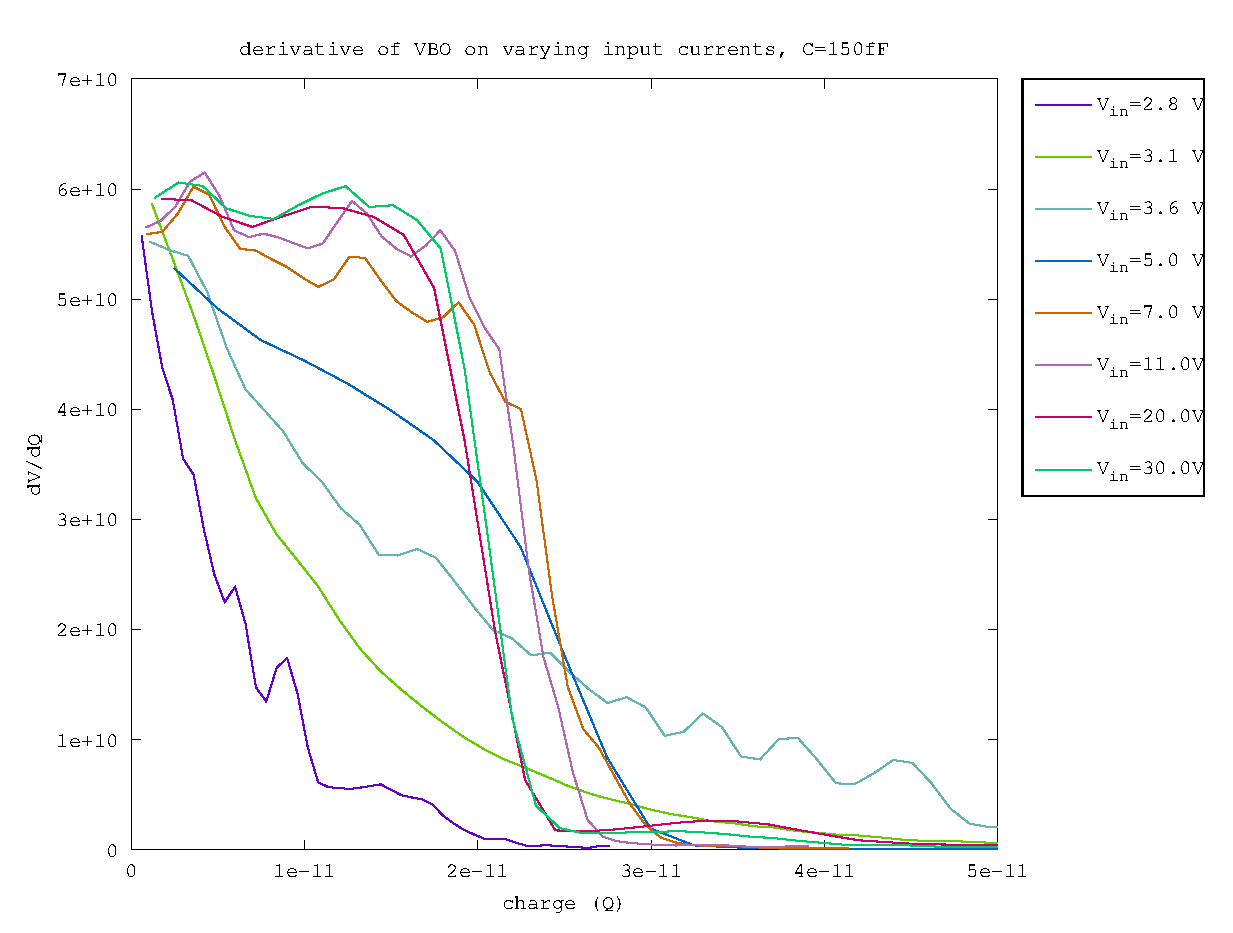
\includegraphics[width=\textwidth]{fig/vbo_d_slope_150fF.eps}
	    \caption[]%
	    {$C=150\,fF$}    
	    \label{fig:vbo_d_slopes_150fF}
	\end{subfigure}
	\quad
	\begin{subfigure}[b]{0.475\textwidth}   
	    \centering 
	    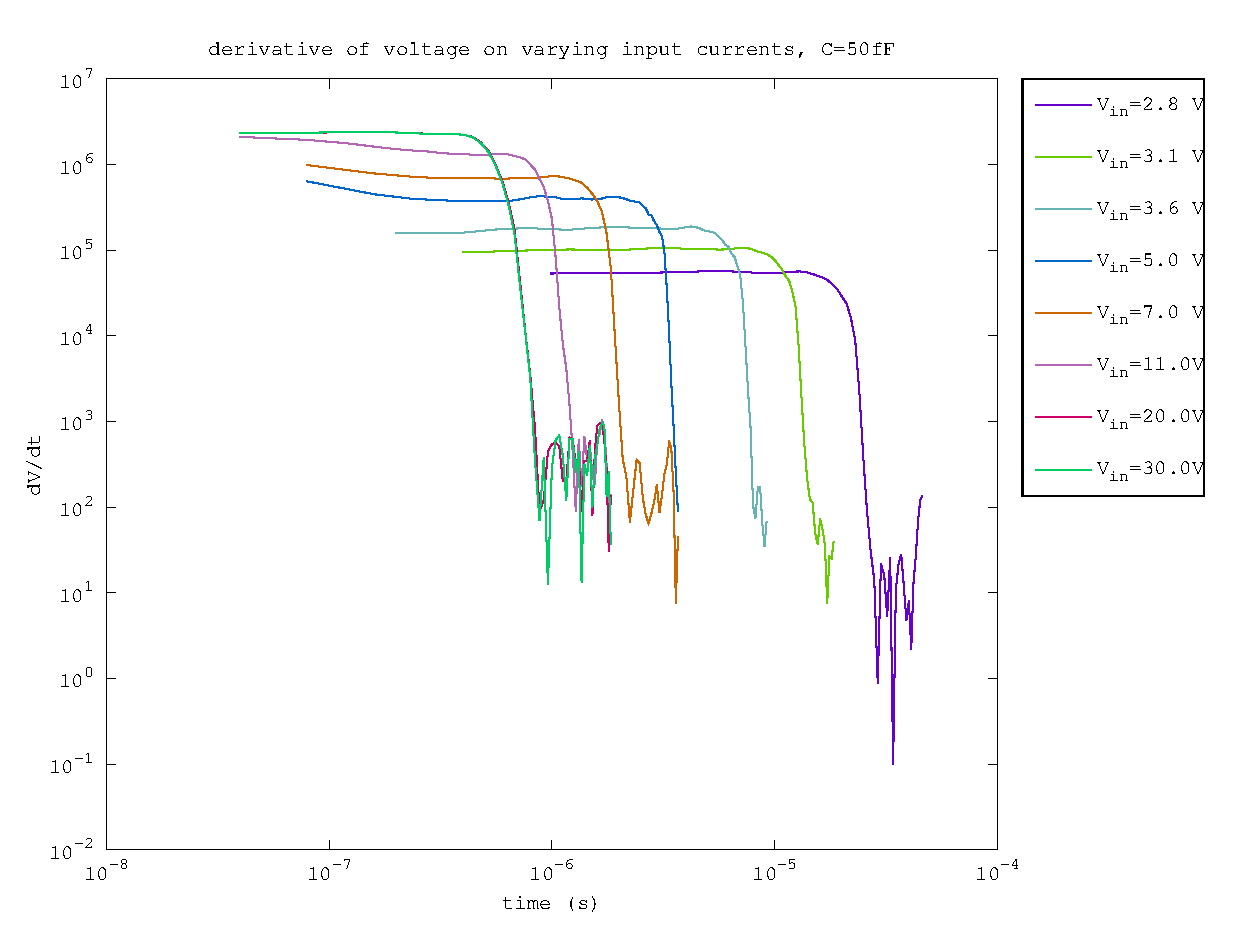
\includegraphics[width=\textwidth]{fig/vbo_d_slope_50fF.eps}
	    \caption[]%
	    {$C=50\,fF$}    
	    \label{fig:vbo_d_slopes_50fF}
	\end{subfigure}
	\caption{The plot shows dv/dt against time of the vbo.}
	\label{fig:vbo_d_slopes}
\end{figure}


\begin{figure}[h]
	\centering
	\begin{subfigure}[b]{0.475\textwidth}
	    \centering
	    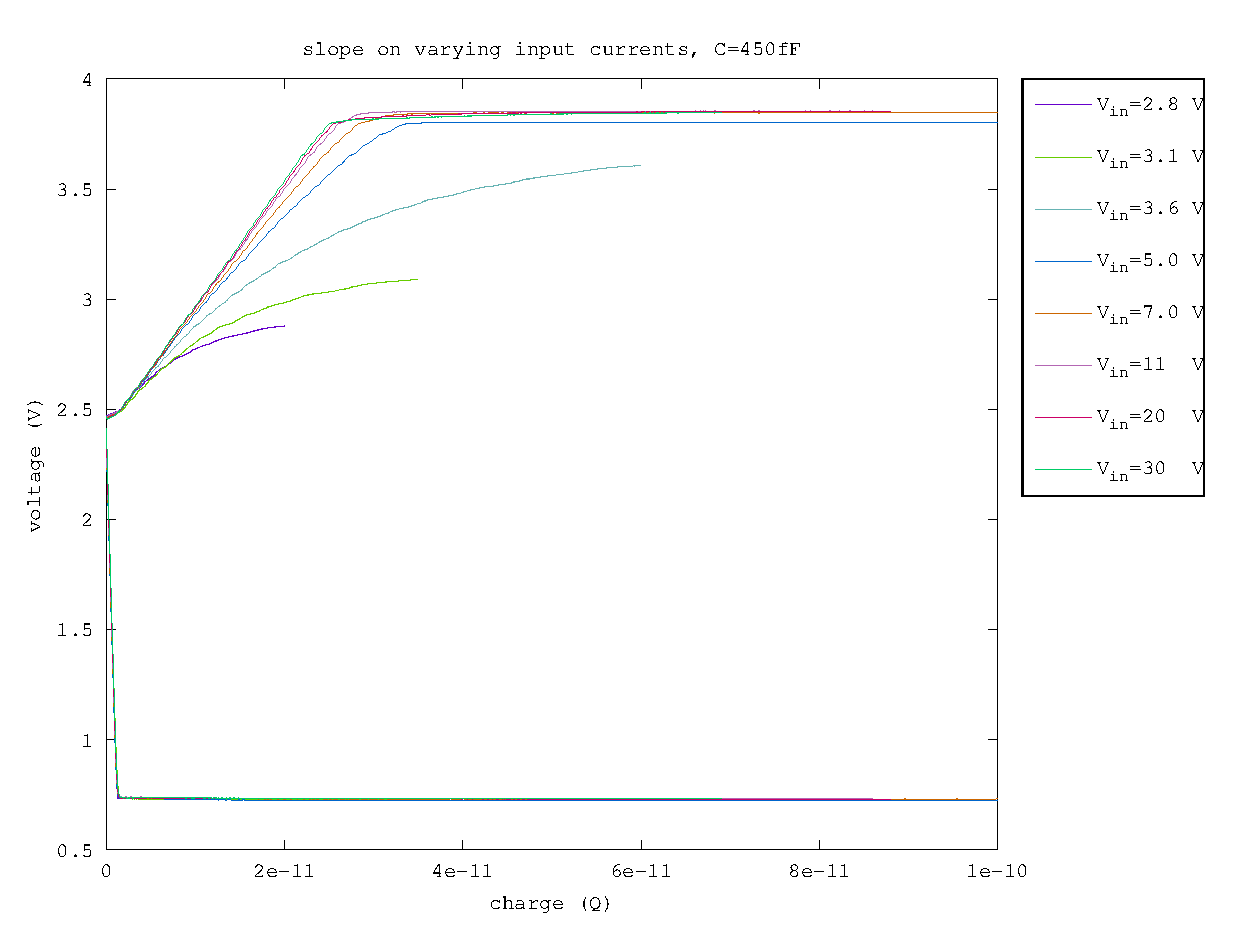
\includegraphics[width=\textwidth]{fig/vbo_charge_450fF.eps}
	    \caption[Network2]%
	    {$C=450\,fF$}    
	    \label{fig:vbo_charges_450fF}
	\end{subfigure}
	\hfill
	\begin{subfigure}[b]{0.475\textwidth}  
	    \centering 
	    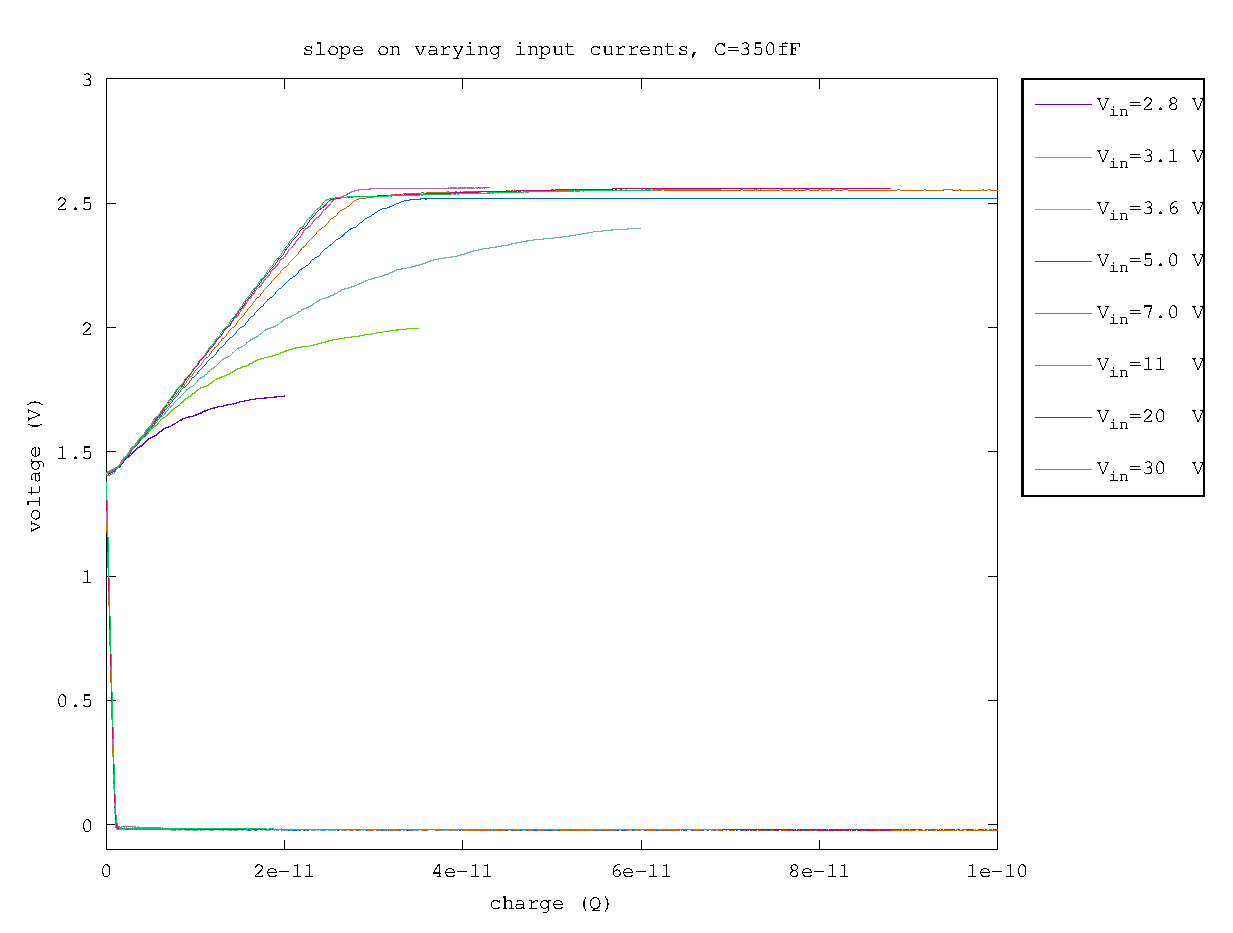
\includegraphics[width=\textwidth]{fig/vbo_charge_350fF.eps}
	    \caption[]%
	    {$C=350\,fF$}    
	    \label{fig:vbo_charges_350fF}
	\end{subfigure}
	\vskip\baselineskip
	\begin{subfigure}[b]{0.475\textwidth}   
	    \centering 
	    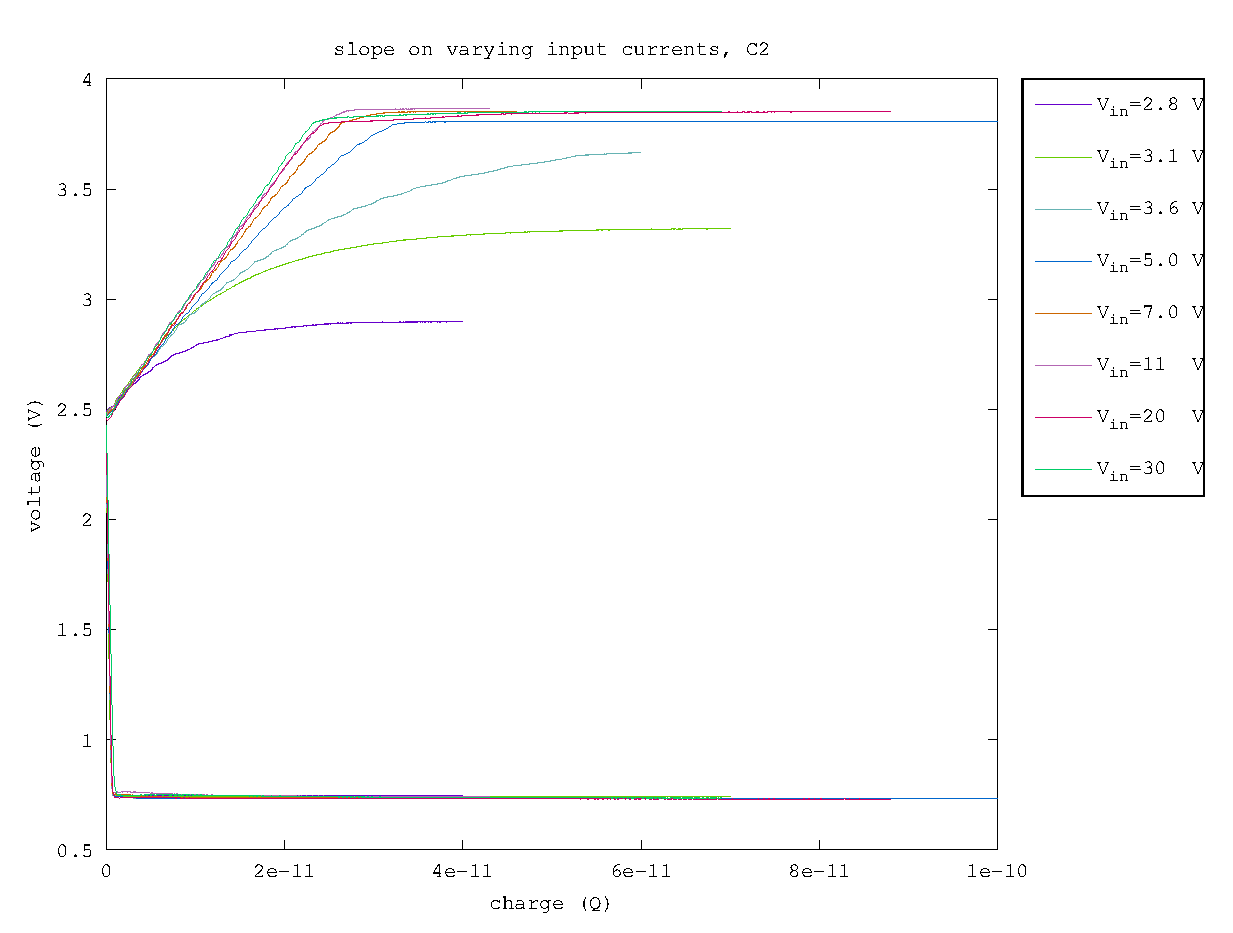
\includegraphics[width=\textwidth]{fig/vbo_charge_150fF.eps}
	    \caption[]%
	    {$C=150\,fF$}    
	    \label{fig:vbo_charges_150fF}
	\end{subfigure}
	\quad
	\begin{subfigure}[b]{0.475\textwidth}   
	    \centering 
	    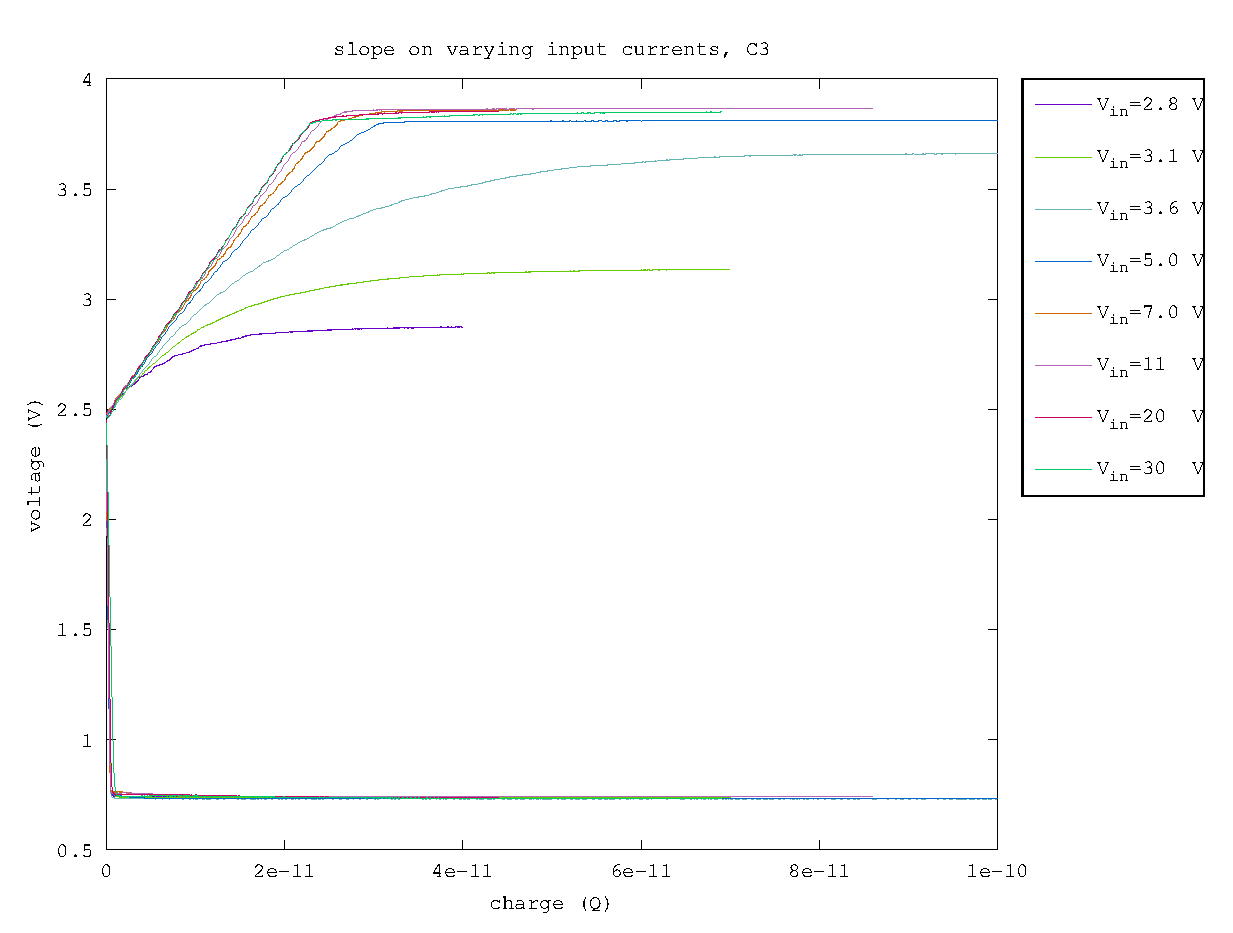
\includegraphics[width=\textwidth]{fig/vbo_charge_50fF.eps}
	    \caption[]%
	    {$C=50\,fF$}    
	    \label{fig:vbo_charges_50fF}
	\end{subfigure}
	\caption{This plot is showing charge versus voltage}
	\label{fig:vbo_charges}
\end{figure}

\begin{figure}[h]
	\centering
	\begin{subfigure}[b]{0.475\textwidth}
	    \centering
	    \includegraphics[width=\textwidth]{fig/vbo_vin_vs_time_sat_450fF.eps}
	    \caption[Network2]%
	    {$C=450\,fF$}    
	    \label{fig:vbo_e_vs_m_450fF}
	\end{subfigure}
	\hfill
	\begin{subfigure}[b]{0.475\textwidth}  
	    \centering 
	    \includegraphics[width=\textwidth]{fig/vbo_vin_vs_time_sat_350fF.eps}
	    \caption[]%
	    {$C=350\,fF$}    
	    \label{fig:vbo_e_vs_m_350fF}
	\end{subfigure}
	\vskip\baselineskip
	\begin{subfigure}[b]{0.475\textwidth}   
	    \centering 
	    \includegraphics[width=\textwidth]{fig/vbo_vin_vs_time_sat_150fF.eps}
	    \caption[]%
	    {$C=150\,fF$}    
	    \label{fig:vbo_e_vs_m_150fF}
	\end{subfigure}
	\quad
	\begin{subfigure}[b]{0.475\textwidth}   
	    \centering 
	    \includegraphics[width=\textwidth]{fig/vbo_vin_vs_time_sat_50fF.eps}
	    \caption[]%
	    {$C=50\,fF$}    
	    \label{fig:vbo_e_vs_m_50fF}
	\end{subfigure}
	\caption{charge times of vbo for different input voltages. The input voltage is connected to the input through a resistor of $20\,M\Omega$.}
	\label{fig:vbo_e_vs_m}
\end{figure}




\clearpage

\end{document}
